% !TeX program = xelatex
\ifdefined\BookMaster\else
\documentclass[11pt,oneside]{article}
% !TeX program = xelatex
\usepackage[b5paper,left=22mm,right=22mm,top=20mm,bottom=22mm,footskip=11mm]{geometry}
\usepackage{fontspec}
\setmainfont{TeX Gyre Termes}
\setsansfont{TeX Gyre Heros}
\usepackage{amsmath,amssymb,mathtools,amsthm}
\renewcommand{\cdots}{\mathinner{\cdotp\cdotp\cdotp}}
\usepackage{graphicx,adjustbox,array,booktabs,longtable,multirow,enumitem,changepage,needspace}
\usepackage[table]{xcolor}
\usepackage{fancyhdr}
\raggedbottom
\interfootnotelinepenalty=10000
\newcommand{\BookFootnote}[2]{\begingroup\renewcommand{\thefootnote}{\fnsymbol{footnote}}\footnote[#1]{#2}\endgroup}
\newcommand{\BookFootnoteMark}[1]{\begingroup\renewcommand{\thefootnote}{\fnsymbol{footnote}}\footnotemark[#1]\endgroup}
\newcommand{\BookFootnoteText}[2]{\begingroup\renewcommand{\thefootnote}{\fnsymbol{footnote}}\footnotetext[#1]{#2}\endgroup}
\newenvironment{BookFloat}[1]{\par\addvspace{.6\baselineskip}\noindent\def\BookFloatID{#1}\begin{minipage}{\linewidth}\phantomsection\label{bookfloat:#1:start}}{\phantomsection\label{bookfloat:\BookFloatID:end}\end{minipage}\par\addvspace{.6\baselineskip}}

\usepackage[unicode,hidelinks]{hyperref}
\pagestyle{fancy}
\fancyhf{}
\newcommand{\BookFooter}{}
\fancyfoot[L]{\parbox[b]{\dimexpr\textwidth-15mm}{\footnotesize\BookFooter}}
\fancyfoot[R]{\footnotesize\thepage}
\renewcommand{\headrulewidth}{0pt}
\renewcommand{\footrulewidth}{0pt}
\setlength{\parindent}{0pt}
\setlength{\parskip}{0.2em}
\setlength{\emergencystretch}{3em}
\setlist{nosep,leftmargin=1.7em,labelsep=.65em}
\newif\ifBookNarrative
\BookNarrativetrue
\newenvironment{BookBody}{\setlength{\parindent}{0pt}}{}
\newcommand{\BookStatement}[1]{\par\addvspace{.6\baselineskip}\noindent #1\enspace\ignorespaces}
\newcommand{\BookLabel}[1]{\par\addvspace{.6\baselineskip}\needspace{3\baselineskip}\noindent\textbf{#1}\quad\ignorespaces}
\newcommand{\BookHeading}[1]{\par\addvspace{\baselineskip}\needspace{4\baselineskip}\noindent{\large\bfseries #1}\par\medskip}
\newcommand{\BookSubheading}[1]{\par\addvspace{.7\baselineskip}\needspace{3\baselineskip}\noindent{\bfseries #1}\par\smallskip}
\newcommand{\BookTextHeading}[1]{\par\addvspace{.7\baselineskip}\needspace{3\baselineskip}\noindent #1\par\smallskip}
\newcommand{\BookSectionTitle}[2]{\par\addvspace{1.2\baselineskip}\needspace{5\baselineskip}\noindent\colorbox{gray!25}{\sffamily\bfseries\small SECTION #1}\quad{\large\bfseries #2}\par\medskip}
\newcommand{\BookExerciseTitle}[1]{\par\addvspace{\baselineskip}\needspace{4\baselineskip}\noindent{\color{gray}\rule{1.5mm}{1.5mm}}\enspace{\large\bfseries Exercises #1}\par\medskip}
\newcommand{\BookBullet}[1]{\begin{list}{\textbullet}{\setlength{\leftmargin}{1.7em}\setlength{\labelwidth}{1em}\setlength{\labelsep}{.7em}\setlength{\topsep}{0pt}\setlength{\parsep}{0pt}\setlength{\itemsep}{0pt}}\item #1\end{list}}
\newcommand{\BookExercise}[2]{\begin{list}{\textbf{#1}}{\setlength{\leftmargin}{2.2em}\setlength{\labelwidth}{1.5em}\setlength{\labelsep}{.7em}\setlength{\topsep}{.15em}\setlength{\parsep}{0pt}\setlength{\itemsep}{0pt}}\item #2\end{list}}
\newcommand{\BookEnd}[1]{\unskip\nobreak\hfill\ensuremath{#1}}
\newcommand{\BookSource}[2]{\phantomsection\label{sourcepage:#1}} % Source-page anchors, retained through reflow.
\usepackage{multicol}
\usepackage{tikz}
\newcommand{\BookPartEntry}[2]{\par\noindent\makebox[17mm][l]{\bfseries Section #1}#2\par}
\newcommand{\BookPartTitle}[3]{\par\bigskip\noindent\begin{tikzpicture}\node[anchor=north west,inner sep=0pt,outer sep=0pt] (bookpart) at (0,0) {\begin{minipage}{\dimexpr\linewidth-.5pt}\hspace*{26mm}\begin{minipage}[t]{\dimexpr\linewidth-26mm}\begin{adjustbox}{max width=\linewidth}{\fontsize{20}{24}\selectfont\bfseries #2}\end{adjustbox}\par\vspace{6mm}\hrule\vspace{6mm}{\sffamily\footnotesize\setlength{\parskip}{.3em}#3}\vspace{3mm}\end{minipage}\end{minipage}};\path[shade,top color=gray!60,bottom color=white] (0,0) rectangle ([xshift=24mm]bookpart.south west);\node[anchor=north,font=\sffamily\bfseries\small] at (12mm,-2mm) {PART};\node[anchor=north,font=\sffamily\bfseries\Huge] at (12mm,-7mm) {#1};\end{tikzpicture}\par\bigskip}
\newsavebox{\BookMathBox}
\makeatletter
\newcommand{\BookInline}[1]{\leavevmode\hskip0pt\relax\begingroup\in@{\begin}{#1}\ifin@\sbox{\BookMathBox}{\(#1\)}\ifdim\wd\BookMathBox>\dimexpr\linewidth-1em\relax\resizebox{\dimexpr\linewidth-1em\relax}{!}{\usebox{\BookMathBox}}\else\(#1\)\fi\else\in@{\left}{#1}\ifin@\sbox{\BookMathBox}{\(#1\)}\ifdim\wd\BookMathBox>\dimexpr\linewidth-1em\relax\resizebox{\dimexpr\linewidth-1em\relax}{!}{\usebox{\BookMathBox}}\else\(#1\)\fi\else\(#1\)\fi\fi\endgroup\hskip0pt\relax}
\makeatother
\DeclareMathOperator{\Aut}{Aut}
\DeclareMathOperator{\End}{End}
\DeclareMathOperator{\Hom}{Hom}
\DeclareMathOperator{\GF}{GF}
\DeclareMathOperator{\irr}{irr}
\DeclareMathOperator{\lt}{lt}
\DeclareMathOperator{\lp}{lp}
\providecommand{\textcircled}[1]{\textnormal{(#1)}}

\begin{document}
\fi
\sloppy
\renewcommand{\BookFooter}{Answers to Odd-Numbered Exercises}
\pdfbookmark[0]{Answers to Odd-Numbered Exercises}{answers}
\ifdefined\BookMaster\else\setcounter{page}{401}\fi
% Source PDF page 418; original printed page 401
\BookSource{418}{401}
\BookNarrativefalse

\begin{BookBody}

\textbf{Answers to Odd-Numbered}

\textbf{Exercises Not Asking for}

\textbf{Definitions or Proofs}

\BookSectionTitle{0}{Sets and Relations}

\BookExercise{3.}{\BookInline{\{1,\allowbreak - 1,\allowbreak 2,\allowbreak - 2,\allowbreak 3,\allowbreak - 3,\allowbreak 4,\allowbreak - 4,\allowbreak 5,\allowbreak - 5,\allowbreak 6,\allowbreak - 6,\allowbreak 10,\allowbreak - 10,\allowbreak 12,\allowbreak - 12,\allowbreak 15,\allowbreak - 15,\allowbreak 20,\allowbreak - 20,\allowbreak 30,\allowbreak - 30,\allowbreak 60,\allowbreak - 60\}}}

\BookExercise{5.}{Not a set (not well defined). A case can also be made for the empty set \BookInline{\emptyset.}}

\BookExercise{7.}{The set \BookInline{\emptyset }}

\BookExercise{9.}{It is not a well-defined set.}

\BookExercise{11.}{\BookInline{(a,\allowbreak 1),\allowbreak (a,\allowbreak 2),\allowbreak (a,\allowbreak c),\allowbreak (b,\allowbreak 1),\allowbreak (b,\allowbreak 2),\allowbreak (b,\allowbreak c),\allowbreak (c,\allowbreak 1),\allowbreak (c,\allowbreak 2),\allowbreak (c,\allowbreak c)}}

\BookExercise{13.}{Draw the line through \BookInline{P} an\BookInline{s}d \BookInline{x,\allowbreak } and let \BookInline{y} be the point where it intersects the line segment \BookInline{CD.}}

\BookExercise{17.}{Conjecture\BookInline{:n(\mathcal{P}(A)_{\aleph })= 2.(}Proofs are usually omitted from answers.)}

\BookExercise{21.}{\BookInline{10^{2},\allowbreak 10^{5},\allowbreak 10^{\aleph _{0}}= 12^{0}= 2^{\aleph _{0}}= |\mathbb{R}|.(}The numbers \BookInline{x} where \BookInline{0\leq x\leq 1} can be written to base 12 and to base 2 as well as to base 10.)}

\BookExercise{23.}{1}

\BookExercise{25.}{5}

\BookExercise{27.}{52}

\BookExercise{29.}{Not an equivalence relation}

\BookExercise{31.}{Not an equivalence relation.}

\BookExercise{33.}{An equivalence relation;}

\begin{center}\begin{adjustbox}{max width=\linewidth}\BookInline{\displaystyle 1= \{1,\allowbreak 2,\allowbreak \cdots ,\allowbreak 9\},\allowbreak }\end{adjustbox}\end{center}

\begin{center}\begin{adjustbox}{max width=\linewidth}\BookInline{\displaystyle 10= \{10,\allowbreak 11,\allowbreak \cdots ,\allowbreak 99\},\allowbreak }\end{adjustbox}\end{center}

\BookInline{100= \{100,\allowbreak 101,\allowbreak \cdots,\allowbreak 999\},\allowbreak } and in general

\begin{center}\begin{adjustbox}{max width=\linewidth}\BookInline{\displaystyle 10^{n}= \{10^{n},\allowbreak 10^{n}+ 1,\allowbreak \cdots ,\allowbreak 10^{n+ 1}- 1\}}\end{adjustbox}\end{center}

\BookExercise{5.}{\textbf{3. a} \BookInline{\{...,\allowbreak - 3,\allowbreak 0,\allowbreak 3,\allowbreak...\},\allowbreak \{...,\allowbreak - 2,\allowbreak 1,\allowbreak 4,\allowbreak...\},\allowbreak \{...,\allowbreak - 5,\allowbreak - 2,\allowbreak 1,\allowbreak...\}}}

\BookExercise{b.}{\BookInline{\{...,\allowbreak - 4,\allowbreak 0,\allowbreak 4,\allowbreak...\},\allowbreak \{...,\allowbreak - 3,\allowbreak 1,\allowbreak 4,\allowbreak...\},\allowbreak \{...,\allowbreak - 6,\allowbreak - 2,\allowbreak 2,\allowbreak...\},\allowbreak \{...,\allowbreak - 5,\allowbreak - 1,\allowbreak 3,\allowbreak...\}}}

\begin{center}\begin{adjustbox}{max width=\linewidth}\BookInline{\displaystyle \mathrm{c}.\{...,\allowbreak - 5,\allowbreak 0,\allowbreak 5,\allowbreak ...\},\allowbreak \{...,\allowbreak - 4,\allowbreak 1,\allowbreak 6,\allowbreak ...\},\allowbreak \{...,\allowbreak - 3,\allowbreak 2,\allowbreak 7,\allowbreak ...\},\allowbreak \{...,\allowbreak - 2,\allowbreak 3,\allowbreak 8...\},\allowbreak \{...,\allowbreak - 1,\allowbreak 4,\allowbreak 9,\allowbreak ...\}}\end{adjustbox}\end{center}

\BookExercise{37.}{\BookInline{1= \{x\in \mathbb{Z}\mid x\div n} has remainder \BookInline{1\}} depends on the value of \BookInline{n.}}

\BookExercise{41.}{The name\textit{ two-to-two function} suggests that such a function \BookInline{f} should carry every pair of distinct points into two distinct points. Such a function is one to one in the conventional sense. (If the domain has only one element, a function cannot fail to be two to two, since the only way it can fail to be two to two is to carry two points into one point, and the set does not have two points.) Conversely, every function that is one to one in the conventional sense carries any pair of points into two distinct points. Thus the functions conventionally called one to one are precisely those that carry two points into two points, which is a much more intuitive unidirectional way of regarding them. Also, the standard way of trying to show a function is one to one is precisely to show that it does not carry two points into just one point. Thus, proving a function is one to one becomes more natural in the two-to-two terminology.}

\end{BookBody}

% Source PDF page 419; original printed page 402
\BookSource{419}{402}
\BookNarrativefalse

\begin{BookBody}

\BookSectionTitle{1}{Binary Operations}

\BookExercise{3.}{\BookInline{a,\allowbreak c.\ast } is not associative.}

\BookExercise{5.}{Top row\BookInline{:d;} second row\BookInline{:a;} fourth row\BookInline{:c,\allowbreak b.}}

\BookExercise{7.}{Not commutative, not associative}

\BookExercise{9.}{Commutative, associative, has identity.}

\BookExercise{11.}{Not commutative, not associative}

\BookExercise{13.}{\BookInline{[n(n+ 1)/2]} \BookInline{8,\allowbreak 729,\allowbreak n}}

\BookExercise{15.}{\BookInline{(n- 1)^{2}} \BookInline{n}}

\BookExercise{19.}{An identity in the set \BookInline{S} with operation \BookInline{\ast } is an element \BookInline{e\in S} such that for all \BookInline{a\in S,\allowbreak a\ast e= e\ast a= a.}}

\BookExercise{21.}{Yes}

\BookExercise{23.}{No. Condition 2 is violated.}

\BookExercise{25.}{No. Condition 1 is violated.}

\BookExercise{7.}{\textbf{2. a} Yes. \textbf{b.} Yes}

\BookExercise{29.}{Let \BookInline{S= \{}?\BookInline{,\allowbreak \Delta \}.} Define \BookInline{\ast } and \BookInline{\ast ^{\prime }} on \BookInline{S} by \BookInline{a\ast b= }? and \BookInline{a\ast ^{\prime }b= \Delta } for all \BookInline{a,\allowbreak b\in S.(}Other answers are possible.)}

\BookExercise{31.}{True}

\BookExercise{33.}{True}

\BookExercise{35.}{False. Let \BookInline{f(x)= x^{2},\allowbreak g(x)= x,\allowbreak } and \BookInline{h(x)= 2x+ 1.} Then}

\begin{center}\begin{adjustbox}{max width=\linewidth}\BookInline{\displaystyle (f(x)- g(x))- h(x)= x^{2}- 3x- 1\;\text{but}\;}\end{adjustbox}\end{center}

\begin{center}\begin{adjustbox}{max width=\linewidth}\BookInline{\displaystyle f(x)- (g(x)- h(x))= x^{2}- (- x- 1)= x^{2}+ x+ 1.}\end{adjustbox}\end{center}

\BookExercise{37.}{True}

\BookExercise{39.}{True}

\BookExercise{41.}{False. Let \BookInline{\ast } be \BookInline{+ } and let \BookInline{\ast ^{\prime }} be on \BookInline{\mathbb{Z}.}}

\BookSectionTitle{2}{Groups}

\BookExercise{1.}{No\BookInline{.\mathcal{G}_{3}} fails.}

\BookExercise{3.}{No\BookInline{.\mathcal{G}_{1}} fails.}

\BookExercise{5.}{No\BookInline{.\mathcal{G}_{1}} fails.}

\BookExercise{7.}{\BookInline{\mathcal{G}_{3}}}

\BookExercise{9.}{\BookInline{\mathcal{G}_{1}}}

\BookExercise{11.}{Yes}

\BookExercise{13.}{Yes}

\BookExercise{15.}{No. The matrix with all entries 0 is upper triangular, but has no inverse.}

\BookExercise{17.}{Yes.}

\BookExercise{19.}{(Proofs are omitted.) \textbf{c}\BookInline{.- 1/3}}

\BookExercise{21.}{2, 3. (It gets harder for 4 elements, where the answer is\textit{ not} 4.)}

\BookExercise{5.}{\textbf{2. a} \BookInline{F} \textbf{c}\BookInline{.T} \textbf{e}\BookInline{.F} \textbf{g}\BookInline{.T} \textbf{i}\BookInline{.F}}

\BookExercise{35.}{2 12 \BookInline{ba}}

\BookSectionTitle{3}{Abelian Examples}

\BookExercise{3.}{\BookInline{- 1}}

\BookExercise{5.}{\BookInline{20- 9i}}

\BookExercise{7.}{\BookInline{17- 15i}}

\BookExercise{9.}{\BookInline{- 4+ 4i}}

\BookInline{\sqrt{2}\left(-\frac{1}{\sqrt{2}}-\frac{1}{\sqrt{2}}i\right)}

\BookExercise{11.}{\BookInline{\sqrt{\pi ^{2}}+ e^{2}}}

\BookExercise{13.}{\BookInline{\sqrt{2}\left(-\frac{1}{\sqrt{2}}-\frac{1}{\sqrt{2}}i\right)}}

\BookInline{\Big(\Big)}

\BookExercise{15.}{\BookInline{\sqrt{34}\left(\frac{-3}{\sqrt{34}}+\frac{5}{\sqrt{34}}i\right)}}

\BookInline{3i,\allowbreak \pm \frac{3\sqrt{3}}{2}-\frac{3}{2}i.}

\BookExercise{17.}{\BookInline{\frac{1}{\sqrt{2}} \pm \frac{1}{\sqrt{2}}i,\allowbreak -\frac{1}{\sqrt{2}} \pm \frac{1}{\sqrt{2}}i.}}

\BookExercise{19.}{\BookInline{3i,\allowbreak \pm \frac{3\sqrt{3}}{2}-\frac{3}{2}i.}}

\BookExercise{21.}{\BookInline{\sqrt{3}\pm i,\allowbreak \pm 2i,\allowbreak - \sqrt{3}\pm i}}

\BookExercise{23.}{7}

\BookExercise{25.}{\BookInline{\frac{3}{8}}}

\BookExercise{27.}{\BookInline{\sqrt{2}}}

\BookExercise{29.}{\BookInline{x= 6}}

\BookExercise{31.}{5}

\BookExercise{33.}{1, 7}

\BookExercise{37.}{\BookInline{\zeta ^{0}\leftrightarrow 0,\allowbreak \zeta ^{3}\leftrightarrow 7,\allowbreak \zeta ^{4}\leftrightarrow 4,\allowbreak \zeta ^{5}\leftrightarrow 1,\allowbreak \zeta ^{6}\leftrightarrow 6,\allowbreak \zeta ^{7}\leftrightarrow 3}}

\BookExercise{39.}{With \BookInline{\zeta \leftrightarrow 4,\allowbreak } we must have \BookInline{\zeta ^{2}\leftrightarrow 2,\allowbreak \zeta ^{3}\leftrightarrow 0,\allowbreak } and \BookInline{\zeta ^{4}\leftrightarrow 4} again, which is impossible for a one-to-one correspondence.}

\BookExercise{41.}{Multiplying, we obtain}

\begin{center}\begin{adjustbox}{max width=\linewidth}\BookInline{\displaystyle z_{1}z_{2}= |z_{1}\parallel z_{2}|[(\;\text{cos}\;\theta _{1}\;\text{cos}\;\theta _{2}- \;\text{sin}\;\theta _{1}\;\text{sin}\;\theta _{2})+ (\;\text{cos}\;\theta _{1}\;\text{sin}\;\theta _{2}+ \;\text{sin}\;\theta _{1}\;\text{cos}\;\theta _{2})i]}\end{adjustbox}\end{center}

and the desired result follows at once from Exercise 40 and the equation \BookInline{|z_{1}||z_{2}|= |z_{1}z_{2}|.}

\BookExercise{45.}{Let \BookInline{f:\mathbb{R}_{b}\to \mathbb{R}_{c}} be given by \BookInline{f(x)= \frac{c}{b}x.}}

\end{BookBody}

% Source PDF page 420; original printed page 403
\BookSource{420}{403}
\BookNarrativefalse

\begin{BookBody}

\BookSectionTitle{4}{Nonabelian Examples}

\BookExercise{1.}{\BookInline{\begin{pmatrix}1 & 2 & 3 & 4 & 5 & 6 \\1 & 2 & 3 & 6 & 5 & 4 \\1 & 2 & 3 & 4 & 5 & 6 \\2 & 6 & 1 & 5 & 4 & 3\end{pmatrix}}}

\BookExercise{3.}{\BookInline{\begin{pmatrix}1 & 2 & 3 & 4 & 5 & 6 \\3 & 4 & 1 & 6 & 2 & 5\end{pmatrix}}}

\BookExercise{5.}{\BookInline{\begin{pmatrix}1 & 2 & 3 & 4 & 5 & 6 \\1 & 2 & 3 & 6 & 5 & 4 \\1 & 2 & 3 & 4 & 5 & 6 \\2 & 6 & 1 & 5 & 4 & 3\end{pmatrix}}}

\BookExercise{7.}{\BookInline{\iota }}

\BookExercise{9.}{\BookInline{\iota }}

\begin{center}\begin{adjustbox}{max width=\linewidth}\BookInline{\displaystyle \begin{aligned} 11.  \quad & \mathbf{a.} \begin{pmatrix}1 & 2 & 3 & 4 & 5 & 6 & 7 & 8 \\4 & 3 & 2 & 5 & 1 & 6 & 7 & 8 \\\end{pmatrix} \\& \mathbf{b.} \begin{pmatrix}1 & 2 & 3 & 4 & 5 & 6 & 7 & 8 \\8 & 6 & 4 & 2 & 1 & 7 & 3 & 5 \\\end{pmatrix} \\& \mathbf{c.} \begin{pmatrix}1 & 2 & 3 & 4 & 5 & 6 & 7 & 8 \\2 & 3 & 1 & 5 & 4 & 7 & 8 & 6 \\\end{pmatrix}\end{aligned}}\end{adjustbox}\end{center}

\BookExercise{3.}{\textbf{1. a} \BookInline{\rho ^{6}} \textbf{b}\BookInline{.\rho } \textbf{c}\BookInline{.\mu \rho ^{10}} \textbf{d}\BookInline{.\mu \rho ^{10}}}

\BookExercise{15.}{\BookInline{\{1,\allowbreak 2,\allowbreak 3,\allowbreak 4,\allowbreak 5,\allowbreak 6\}}}

\BookExercise{17.}{\BookInline{\{1,\allowbreak 5\}}}

\BookExercise{9.}{\textbf{1. a} These are “elementary permutation matrices,” resulting from permuting the rows of the identity matrix. When another matrix \BookInline{A} is multiplied on the left by one of these matrices \BookInline{P,\allowbreak } the rows of \BookInline{A} are permuted in the same fashion that the rows of the \BookInline{3\times 3} identity matrix were permuted to obtain \BookInline{P.} Because all 6 possible permutations of the three rows are present, we see they will act just like the elements of \BookInline{S_{3}} in permuting the entries 1, 2, 3 of the given column vector. Thus they form a group because \BookInline{S_{3}} is a group.}

\BookExercise{b.}{The symmetric group \BookInline{S_{3}.}}

\BookExercise{21.}{Need to add that \BookInline{\phi } is one-to-one and onto.}

\BookExercise{23.}{This is a good definition.}

\BookExercise{25.}{Not a permutation}

\BookExercise{27.}{Not a permutation}

\BookExercise{9.}{\textbf{2. a} \BookInline{T} \textbf{c}\BookInline{.T} \textbf{e}\BookInline{.F} \textbf{g}\BookInline{.F}}

\BookSectionTitle{5}{Subgroups}

\BookExercise{3.}{Yes}

\BookExercise{5.}{Yes}

\BookExercise{7.}{\BookInline{\mathbb{Q}^{+ }} and \BookInline{\{\pi ^{n}\mid n\in \mathbb{Z}\}}}

\BookExercise{9.}{Yes}

\BookExercise{11.}{No. Not closed under multiplication.}

\BookExercise{13.}{Yes}

\BookExercise{5.}{\textbf{1. a} Yes \textbf{b.} No. It is not even a subset of F\BookInline{˜.}}

\BookExercise{7.}{\textbf{1. a} No. Not closed under addition. \textbf{b.} Yes}

\BookExercise{9.}{\textbf{1. a} Yes \textbf{b.} No. The zero constant function is not in F\BookInline{˜.}}

\BookExercise{21.}{\BookInline{\iota,\allowbreak \rho ^{3},\allowbreak \rho ^{6},\allowbreak \rho ^{9},\allowbreak \rho ^{12},\allowbreak \rho ^{15}}}

\BookExercise{1.}{\textbf{2. a} \BookInline{- 50,\allowbreak - 25,\allowbreak 0,\allowbreak 25,\allowbreak 50} \textbf{b.} 4, 2, 1, 1/2, 1/4 \textbf{c}\BookInline{.1,\allowbreak \pi,\allowbreak \pi ^{2},\allowbreak 1/\pi,\allowbreak 1/\pi ^{2}} \textbf{e}\BookInline{.\iota,\allowbreak (1,\allowbreak 2,\allowbreak 3)(5,\allowbreak 6),\allowbreak (1,\allowbreak 3,\allowbreak 2),\allowbreak (5,\allowbreak 6),\allowbreak (1,\allowbreak 2,\allowbreak 3),\allowbreak (1,\allowbreak 3,\allowbreak 2)(5,\allowbreak 6)}}

\BookInline{\Big[\Big]}

\BookExercise{23.}{All matrices \BookInline{\begin{bmatrix} 1 & n \\ 0 & 1 \end{bmatrix}} for \BookInline{n\in \mathbb{Z}}}

\BookInline{\Big[\Big]\Big[\Big]}

\BookExercise{25.}{All matrices of the form \BookInline{\begin{bmatrix} 4^{n} & 0 \\ 0 & 4^{n} \end{bmatrix} or \begin{bmatrix} 0 & -2^{2n+1} \\ -2^{2n+1} & 0 \end{bmatrix}} for \BookInline{n\in \mathbb{Z}}}

\BookExercise{27.}{4}

\BookExercise{29.}{3}

\BookExercise{31.}{4}

\BookExercise{33.}{2}

\BookExercise{35.}{3}

\BookExercise{9.}{\textbf{3. a} \BookInline{T} \textbf{c}\BookInline{.T} \textbf{e}\BookInline{.F} \textbf{g}\BookInline{.F} \textbf{i}\BookInline{.T}}

\BookExercise{41.}{This is a subgroup\BookInline{:\iota } is in the set, the set is closed under function composition, and if \BookInline{\sigma (b)= b,\allowbreak } then \BookInline{\sigma ^{- 1}(b)= b.}}

\BookExercise{43.}{This is not a subgroup. Let \BookInline{A= \mathbb{Z},\allowbreak B= \mathbb{Z}^{+ },\allowbreak } and \BookInline{b= 1.} The permutation \BookInline{\sigma (n)= n+ 1} mapping \BookInline{\mathbb{Z}} to \BookInline{\mathbb{Z}} is in the set, but \BookInline{\sigma ^{- 1}} is not in the set.}

\BookSectionTitle{6}{Cyclic Groups}

\BookExercise{3.}{\BookInline{q= - 5,\allowbreak r= 3}}

\BookExercise{5.}{8}

\BookExercise{7.}{60}

\BookExercise{9.}{\BookInline{4}}

\BookExercise{11.}{\BookInline{24}}

\BookExercise{13.}{2}

\BookExercise{15.}{2}

\BookExercise{17.}{6}

\BookExercise{19.}{4}

\BookExercise{21.}{An infinite cyclic group}

\BookExercise{23.}{75}

\BookExercise{25.}{6}

\BookExercise{27.}{12}

\BookExercise{29.}{30}

\end{BookBody}

% Source PDF page 421; original printed page 404
\BookSource{421}{404}
\BookNarrativefalse

\begin{BookBody}

\begin{BookFloat}{answers-p421-1}
\begin{center}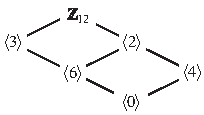
\includegraphics[width=0.280\linewidth,height=.8\textheight,keepaspectratio]{assets/p421_01.pdf}\end{center}
\end{BookFloat}

\BookExercise{33.}{8}

\begin{center}\begin{adjustbox}{max width=\linewidth}\BookInline{\displaystyle \langle 2\rangle}\end{adjustbox}\end{center}

\BookInline{\langle 4\rangle }

\BookInline{\langle 0\rangle }

\BookExercise{1.}{\textbf{4. a} \BookInline{T} \textbf{c}\BookInline{.F} \textbf{e}\BookInline{.T} \textbf{g}\BookInline{.F} \textbf{i}\BookInline{.T}}

\BookExercise{43.}{\BookInline{<Q,\allowbreak + >}}

\BookExercise{45.}{ There is none.}

\BookInline{\textstyle { \frac { \sqrt { 2 } } { 2 } } ( \pm 1 \pm i )}

\BookExercise{47.}{\BookInline{i,\allowbreak - i}}

\BookExercise{49.}{\BookInline{\textstyle { \frac { \sqrt { 2 } } { 2 } } ( \pm 1 \pm i )}}

\BookExercise{63.}{\BookInline{(p- 1)p^{r- 1}}}

\BookSectionTitle{7}{Generating Sets and Cayley Digraphs}

\BookExercise{3.}{\BookInline{\mathbb{Z}} 25}

\BookExercise{5.}{\BookInline{\cdots,\allowbreak - 24,\allowbreak - 18,\allowbreak - 12,\allowbreak - 6,\allowbreak 0,\allowbreak 6,\allowbreak 12,\allowbreak 18,\allowbreak 24,\allowbreak \cdots }}

\BookExercise{7.}{\BookInline{\{\iota,\allowbreak \rho ^{2},\allowbreak \rho ^{4},\allowbreak \rho ^{6},\allowbreak \mu,\allowbreak \mu \rho ^{2},\allowbreak \mu \rho ^{4},\allowbreak \mu \rho ^{6}\}}}

\BookExercise{9.}{\textbf{. a} \BookInline{c} \textbf{b}\BookInline{.e} \textbf{c}\BookInline{.d}}

\begin{BookFloat}{answers-p421-22}
\begin{center}\begin{adjustbox}{max width=\linewidth}
\renewcommand{\arraystretch}{1.2}\setlength{\tabcolsep}{5pt}
\begin{tabular}{c|c|c|c|c|c|c}
 & \BookInline{e} & \BookInline{a} & \BookInline{b} & \BookInline{c} & \BookInline{d} & \BookInline{f}\\\hline
\BookInline{e} & \BookInline{e} & \BookInline{a} & \BookInline{b} & \BookInline{c} & \BookInline{d} & \BookInline{f}\\\hline
\BookInline{a} & \BookInline{a} & \BookInline{e} & \BookInline{c} & \BookInline{b} & \BookInline{f} & \BookInline{d}\\\hline
\BookInline{b} & \BookInline{b} & \BookInline{d} & \BookInline{e} & \BookInline{f} & \BookInline{a} & \BookInline{c}\\\hline
\BookInline{c} & \BookInline{c} & \BookInline{f} & \BookInline{a} & \BookInline{d} & \BookInline{e} & \BookInline{b}\\\hline
\BookInline{d} & \BookInline{d} & \BookInline{b} & \BookInline{f} & \BookInline{e} & \BookInline{c} & \BookInline{a}\\\hline
\BookInline{f} & \BookInline{f} & \BookInline{c} & \BookInline{d} & \BookInline{a} & \BookInline{b} & \BookInline{e}\\
\end{tabular}
\end{adjustbox}\end{center}
\end{BookFloat}

\BookExercise{13.}{Choose a pair of generating directed arcs, call them\textit{ arc1} and\textit{ arc2}, start at any vertex of the digraph, and see if the sequences\textit{ arc1},\textit{ arc2} and\textit{ arc2},\textit{ arc1} lead to the same vertex. (This corresponds to asking if the two corresponding group generators commute.) The group is commutative if and only if these two sequences lead to the same vertex for \textit{every pair} of generating directed arcs.}

\BookExercise{15.}{It is not obvious, since a digraph of a cyclic group might be formed using a generating set of two or more elements, no one of which generates the group.}

\begin{BookFloat}{answers-p421-25}
\begin{center}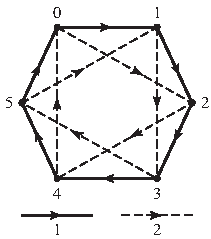
\includegraphics[width=0.289\linewidth,height=.8\textheight,keepaspectratio]{assets/p421_19.pdf}\end{center}
\end{BookFloat}

\BookExercise{9.}{\textbf{1. a} Starting from any vertex \BookInline{a,\allowbreak } every path through the graph that terminates at that same vertex \BookInline{a} represents a product of generators or their inverses that is equal to the identity and thus gives a relation.}

\BookExercise{b.}{\textbf{b}\BookInline{.a^{4}= e,\allowbreak b^{2}= e,\allowbreak (ab)^{2}= e}}

\end{BookBody}

% Source PDF page 422; original printed page 405
\BookSource{422}{405}
\BookNarrativefalse

\begin{BookBody}

\BookSectionTitle{8}{Groups of Permutations}

\BookExercise{3.}{Homomorphism}

\BookExercise{5.}{Not a homomorphism}

\BookExercise{7.}{Homomorphism}

\BookExercise{9.}{Not a homomorphism}

\BookExercise{11.}{Ker\BookInline{(\phi )= \langle 4\rangle.}}

\BookExercise{13.}{Ker\BookInline{(\phi )= \langle (5,\allowbreak 3)\rangle.}}

\BookExercise{15.}{\BookInline{\{0,\allowbreak 0\}}}

\BookExercise{17.}{\BookInline{\{1,\allowbreak 2,\allowbreak 5\},\allowbreak \{3\},\allowbreak \{4,\allowbreak 6\}}}

\BookExercise{19.}{\BookInline{\{1,\allowbreak 2,\allowbreak 3,\allowbreak 4,\allowbreak 5\},\allowbreak \{6\},\allowbreak \{7,\allowbreak 8\}}}

\BookExercise{21.}{\BookInline{\{2n\mid n\in \mathbb{Z}\},\allowbreak \{2n+ 1\mid n\in \mathbb{Z}\}}}

\BookExercise{23.}{\BookInline{(1,\allowbreak 8)(3,\allowbreak 6,\allowbreak 4)(5,\allowbreak 7)= (1,\allowbreak 8)(3,\allowbreak 4)(3,\allowbreak 6)(5,\allowbreak 7)}}

\BookExercise{25.}{\BookInline{(1,\allowbreak 5,\allowbreak 4,\allowbreak 8)(2,\allowbreak 3)(6,\allowbreak 7)= (1,\allowbreak 8)(1,\allowbreak 4)(1,\allowbreak 5)(2,\allowbreak 3)(6,\allowbreak 7)}}

\BookExercise{1.}{\textbf{3. a} \BookInline{F} \textbf{c}\BookInline{.F} \textbf{e}\BookInline{.F} \textbf{g}\BookInline{.T} \textbf{i}\BookInline{.T} \textbf{k}\BookInline{.T}}

\BookSectionTitle{9}{Finitely Generated Abelian Groups}

\begin{BookFloat}{answers-p422-17}
\noindent\textbf{1.}\quad
\begin{tabular}{cc|cc}
\textit{Element}&\textit{Order}&\textit{Element}&\textit{Order}\\
$(0,0)$&1&$(0,2)$&2\\
$(1,0)$&2&$(1,2)$&2\\
$(0,1)$&4&$(0,3)$&4\\
$(1,1)$&4&$(1,3)$&4
\end{tabular}
\end{BookFloat}

The group is not cyclic

\BookExercise{3.}{2}

\BookExercise{5.}{9}

\BookExercise{7.}{60}

\BookExercise{9.}{\BookInline{\{(0,\allowbreak 0),\allowbreak (0,\allowbreak 1)\},\allowbreak \{(0,\allowbreak 0),\allowbreak (1,\allowbreak 0)\},\allowbreak \{(0,\allowbreak 0),\allowbreak (1,\allowbreak 1)\}}}

\BookExercise{11.}{\BookInline{\{(0,\allowbreak 0),\allowbreak (0,\allowbreak 1),\allowbreak (0,\allowbreak 2),\allowbreak (0,\allowbreak 3)\}} \BookInline{\{(0,\allowbreak 0),\allowbreak (0,\allowbreak 2),\allowbreak (1,\allowbreak 0),\allowbreak (1,\allowbreak 2)\}} \BookInline{\{(0,\allowbreak 0),\allowbreak (1,\allowbreak 1),\allowbreak (0,\allowbreak 2),\allowbreak (1,\allowbreak 3)\}}}

\BookExercise{13.}{\BookInline{\mathbb{Z}_{20}\times \mathbb{Z}_{3},\allowbreak \mathbb{Z}_{15}\times \mathbb{Z}_{4},\allowbreak \mathbb{Z}_{12}\times \mathbb{Z}_{5},\allowbreak \mathbb{Z}_{5}\times \mathbb{Z}_{3}\times \mathbb{Z}_{4}}}

\BookExercise{15.}{12}

\BookExercise{17.}{168}

\BookExercise{19.}{180}

\BookExercise{21.}{\BookInline{\mathbb{Z}_{8},\allowbreak \mathbb{Z}_{2}\times \mathbb{Z}_{4},\allowbreak \mathbb{Z}_{2}\times \mathbb{Z}_{2}\times \mathbb{Z}_{2}}}

\BookExercise{23.}{\BookInline{\mathbb{Z}_{32},\allowbreak \mathbb{Z}_{2}\times \mathbb{Z}_{16},\allowbreak \mathbb{Z}_{4}\times \mathbb{Z}_{8},\allowbreak \mathbb{Z}_{2}\times \mathbb{Z}_{2}\times \mathbb{Z}_{8},\allowbreak \mathbb{Z}_{2}\times \mathbb{Z}_{4}\times \mathbb{Z}_{4},\allowbreak }}

\begin{center}\begin{adjustbox}{max width=\linewidth}\BookInline{\displaystyle \mathbb{Z}_{2}\times \mathbb{Z}_{2}\times \mathbb{Z}_{2}\times \mathbb{Z}_{4},\allowbreak \mathbb{Z}_{2}\times \mathbb{Z}_{2}\times \mathbb{Z}_{2}\times \mathbb{Z}_{2}\times \mathbb{Z}_{2}}\end{adjustbox}\end{center}

\BookExercise{25.}{\BookInline{\mathbb{Z}_{9}\times \mathbb{Z}_{121},\allowbreak \mathbb{Z}_{3}\times \mathbb{Z}_{3}\times \mathbb{Z}_{121},\allowbreak \mathbb{Z}_{9}\times \mathbb{Z}_{11}\times \mathbb{Z}_{11},\allowbreak \mathbb{Z}_{3}\times \mathbb{Z}_{3}\times \mathbb{Z}_{11}\times \mathbb{Z}_{11}}}

\begin{BookFloat}{answers-p422-32}
\BookExercise{29. a.}{\begin{tabular}{r|ccccccc}
$n$&2&3&4&5&6&7&8\\\hline
number of groups&2&3&5&7&11&15&22
\end{tabular}}
\end{BookFloat}

\BookExercise{b.}{\textbf{b. i)} 225 \textbf{ii)} 225 \textbf{iii)} 110}

\BookExercise{1.}{\textbf{3. a} It is abelian when the arrows on both \BookInline{n-}gons have the same (clockwise or counterclockwise) direction. \textbf{b}\BookInline{.\mathbb{Z}_{2}\times \mathbb{Z}_{n}} \textbf{c.} When \BookInline{n} is odd. \textbf{d.} The dihedral group \BookInline{D_{n}.}}

\BookExercise{33.}{\BookInline{\mathbb{Z}_{2}} is an example.}

\BookExercise{35.}{\BookInline{S_{3}} is an example.}

\BookExercise{37.}{The numbers are the same.}

\BookExercise{41.}{\BookInline{\{- 1,\allowbreak 1\}}}

\end{BookBody}

% Source PDF page 423; original printed page 406
\BookSource{423}{406}
\BookNarrativefalse

\begin{BookBody}

\BookSectionTitle{10}{Cosets and the Theorem of Lagrange}

\begin{center}\begin{adjustbox}{max width=\linewidth}\BookInline{\displaystyle 1+ 4\mathbb{Z}= \{\cdots ,\allowbreak - 7,\allowbreak - 3,\allowbreak 1,\allowbreak 5,\allowbreak 9,\allowbreak \cdots \}}\end{adjustbox}\end{center}

\begin{center}\begin{adjustbox}{max width=\linewidth}\BookInline{\displaystyle 2+ 4\mathbb{Z}= \{\cdots ,\allowbreak - 6,\allowbreak - 2,\allowbreak 2,\allowbreak 6,\allowbreak 10,\allowbreak \cdots \}}\end{adjustbox}\end{center}

\begin{center}\begin{adjustbox}{max width=\linewidth}\BookInline{\displaystyle 3+ 4\mathbb{Z}= \{\cdots ,\allowbreak - 5,\allowbreak - 1,\allowbreak 3,\allowbreak 7,\allowbreak 11,\allowbreak \cdots \}}\end{adjustbox}\end{center}

\BookExercise{3.}{\BookInline{\{0,\allowbreak 3,\allowbreak 6,\allowbreak 9,\allowbreak 12,\allowbreak 15\},\allowbreak \{1,\allowbreak 4,\allowbreak 7,\allowbreak 10,\allowbreak 13,\allowbreak 16\},\allowbreak \{2,\allowbreak 5,\allowbreak 8,\allowbreak 11,\allowbreak 14,\allowbreak 17\}}}

\BookExercise{5.}{\BookInline{\langle 18\rangle = \{0,\allowbreak 18\},\allowbreak 1+ \langle 18\rangle = \{1,\allowbreak 19\},\allowbreak 2+ \langle 18\rangle = \{2,\allowbreak 20\},\allowbreak \cdots,\allowbreak 17+ \langle 18\rangle = \{17,\allowbreak 35\}}}

\BookExercise{7.}{\BookInline{\{\iota,\allowbreak \mu \rho \},\allowbreak \{\rho,\allowbreak \mu \rho ^{2}\},\allowbreak \{\rho ^{2},\allowbreak \mu \rho ^{3}\},\allowbreak \{\rho ^{3},\allowbreak \mu \}} They are different.}

\BookExercise{9.}{\BookInline{\{\iota,\allowbreak \rho ^{2}\},\allowbreak \{\rho,\allowbreak \rho ^{3}\},\allowbreak \{\mu,\allowbreak \mu \rho ^{2}\},\allowbreak \{\mu \rho,\allowbreak \mu \rho ^{3}\}}}

\BookExercise{11.}{4}

\BookExercise{13.}{12}

\BookExercise{15.}{24}

\BookExercise{21.}{\BookInline{2\mathbb{Z}\leq \mathbb{Z}} has only 2 cosets.}

\BookExercise{23.}{\BookInline{G= \mathbb{Z}_{2},\allowbreak } subgroup \BookInline{H= \mathbb{Z}_{2}.}}

\BookExercise{25.}{Impossible. The number of cells must divide the order of the group, and 12 does not divide 6.}

\BookSectionTitle{11}{Plane Isometries}

\BookExercise{1.}{\textbf{. a} The only isometries of \BookInline{\mathbb{R}} leaving a number \BookInline{c} fixed are the reflection through \BookInline{c} that carries \BookInline{c+ x} to \BookInline{c- x} for all \BookInline{x\in \mathbb{R},\allowbreak } and the identity map.}

\BookExercise{b.}{The isometries of \BookInline{\mathbb{R}^{2}} that leave a point \BookInline{P} fixed are the rotations about \BookInline{P} through any angle \BookInline{\theta } where \BookInline{0\leq \theta <360^{\circ }} and the reflections across any axis that passes through \BookInline{P.}}

\BookExercise{c.}{The only isometries of \BookInline{\mathbb{R}} that carry a line segment into itself are the reflection through the midpoint of the line segment (see the answer to part (a)) and the identity map.}

\BookExercise{d.}{The isometries of \BookInline{\mathbb{R}^{2}} that carry a line segment into itself are a rotation of \BookInline{180^{\circ }} about the midpoint of the line segment, a reflection in the axis containing the line segment, a reflection in the axis perpendicular to the line segment at its midpoint, and the identity map.}

\BookExercise{e.}{The isometries of \BookInline{\mathbb{R}^{3}} that carry a line segment into itself include rotations through any angle about an axis that contains the line segment, reflections across any plane that contains the line segment, and reflection across the plane perpendicular to the line segment at its midpoint.}

\begin{BookFloat}{answers-p423-23}
\begin{center}\begin{adjustbox}{max width=\linewidth}
\renewcommand{\arraystretch}{1.2}\setlength{\tabcolsep}{5pt}
\begin{tabular}{c|c|c|c|c}
 & \BookInline{\tau } & \BookInline{\rho } & \BookInline{\mu } & \BookInline{\gamma }\\\hline
\BookInline{\tau } & \BookInline{\tau } & \BookInline{\rho } & \BookInline{\mu \gamma } & \BookInline{\mu \gamma }\\\hline
\BookInline{\rho } & \BookInline{\rho } & \BookInline{\rho \tau } & \BookInline{\mu \gamma } & \BookInline{\mu \gamma }\\\hline
\BookInline{\mu } & \BookInline{\mu \gamma } & \BookInline{\mu \gamma } & \BookInline{\tau \rho } & \BookInline{\tau \rho }\\\hline
\BookInline{\gamma } & \BookInline{\mu \gamma } & \BookInline{\mu \gamma } & \BookInline{\tau \rho } & \BookInline{\tau \rho }\\
\end{tabular}
\end{adjustbox}\end{center}
\end{BookFloat}

\begin{BookFloat}{answers-p423-24}
\begin{center}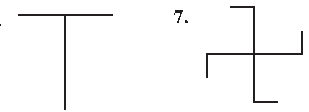
\includegraphics[width=0.424\linewidth,height=.8\textheight,keepaspectratio]{assets/p423_23.pdf}\end{center}
\end{BookFloat}

\BookExercise{9.}{\textit{Translation:} order \BookInline{\infty }}

\textit{Rotation:} order any \BookInline{n\geq 2} or \BookInline{\infty }

\textit{Reflection:} order 2

\textit{Glide reflection:} order \BookInline{\infty }

\BookExercise{11.}{Rotations}

\BookExercise{13.}{Only the identity and reflections.}

\BookExercise{17.}{Yes. The product of two translations is a translation and the inverse of a translation is a translation.}

\BookExercise{19.}{Yes. There is only one reflection \BookInline{\mu } across one particular line \BookInline{L,\allowbreak } and \BookInline{\mu ^{2}} is the identity, so we have a group isomorphic to \BookInline{\mathbb{Z}_{2}.}}

\end{BookBody}

% Source PDF page 424; original printed page 407
\BookSource{424}{407}
\BookNarrativefalse

\begin{BookBody}

\BookExercise{21.}{Only reflections and rotations (and the identity) because translations and glide reflections do not have finite order in the group of all plane isometries.}

\BookExercise{5.}{\textbf{2. a} No \textbf{b.} No \textbf{c.} Yes \textbf{d.} No \textbf{e}\BookInline{.D_{\infty }}}

\BookExercise{7.}{\textbf{2. a} Yes \textbf{b.} No \textbf{c.} No \textbf{d.} No \textbf{e}\BookInline{.D_{\infty }}}

\BookExercise{9.}{\textbf{2. a} No \textbf{b.} No \textbf{c.} No \textbf{d.} Yes \textbf{e}\BookInline{.\mathbb{Z}}}

\BookExercise{1.}{\textbf{3. a} Yes\BookInline{.90^{\circ },\allowbreak 180^{\circ }} \textbf{b.} Yes \textbf{c.} No}

\BookExercise{3.}{\textbf{3. a} No \textbf{b.} No \textbf{c.} No}

\BookExercise{5.}{\textbf{3. a} Yes\BookInline{.180^{\circ }} \textbf{b.} Yes \textbf{c.} No}

\BookExercise{7.}{\textbf{3. a} Yes\BookInline{.120^{\circ }} \textbf{b.} Yes \textbf{c.} No}

\BookExercise{9.}{\textbf{3. a} Yes\BookInline{.120^{\circ }} \textbf{b.} No \textbf{c.} No \textbf{d}\BookInline{.(1,\allowbreak 0),\allowbreak (1,\allowbreak \sqrt{3})}}

\BookSectionTitle{12}{Factor Groups}

\BookExercise{3.}{4}

\BookExercise{5.}{3}

\BookExercise{7.}{1}

\BookExercise{9.}{4}

\BookExercise{11.}{3}

\BookExercise{13.}{5}

\BookExercise{15.}{1}

\BookExercise{1.}{\textbf{2. a} When working with a factor group \BookInline{G/H,\allowbreak } you would let \BookInline{a} and \BookInline{b} be elements of \BookInline{G,\allowbreak } not elements of \BookInline{G/H.} The student probably does not understand what elements of \BookInline{G/H} look like and can write nothing sensible concerning them.}

\BookExercise{b.}{We must show that \BookInline{G/H} is abelian. Let \BookInline{aH} and \BookInline{bH} be two elements of \BookInline{G/H.}}

\BookExercise{3.}{\textbf{2. a} \BookInline{T} \textbf{c}\BookInline{.T} \textbf{e}\BookInline{.T} \textbf{g}\BookInline{.T} \textbf{i}\BookInline{.T}}

\BookExercise{35.}{Example: Let \BookInline{G= N= S_{3},\allowbreak } and let \BookInline{H= \{\rho _{0},\allowbreak \mu _{1}\}.} Then \BookInline{N} is normal in \BookInline{G,\allowbreak } but \BookInline{H\cap N= H} is not normal in \BookInline{G.}}

\BookSectionTitle{13}{Factor-Group Computations and Simple Groups}

\BookExercise{3.}{\BookInline{\mathbb{Z}_{4}}}

\BookExercise{5.}{\BookInline{\mathbb{Z}_{4}\times \mathbb{Z}_{8}}}

\BookExercise{7.}{\BookInline{\mathbb{Z}\times \mathbb{Z}_{2}}}

\BookExercise{9.}{\BookInline{\mathbb{Z}_{3}\times \mathbb{Z}\times \mathbb{Z}_{4}}}

\BookExercise{11.}{\BookInline{\mathbb{Z}_{2}\times \mathbb{Z}}}

\BookExercise{13.}{\BookInline{\mathbb{Z}\times \mathbb{Z}_{2}}}

\BookExercise{15.}{\BookInline{Z(D_{4})= C= \{\iota,\allowbreak \rho ^{2}\}}}

\BookExercise{17.}{\BookInline{Z(S_{3}\times D_{4})= \{\{\iota,\allowbreak \iota \},\allowbreak \{\iota,\allowbreak \rho \}\},\allowbreak C= A_{3}\times \{\iota,\allowbreak \rho \}.}}

\BookExercise{1.}{\textbf{2. a} \BookInline{T} \textbf{c}\BookInline{.F} \textbf{e}\BookInline{.F} \textbf{g}\BookInline{.F} \textbf{i}\BookInline{.T}}

\BookExercise{23.}{\BookInline{\{f\in F^{\ast }\mid f(0)= 1\}}}

\BookExercise{25.}{Yes. Let \BookInline{f(x)= 1} for \BookInline{x\geq 0} and \BookInline{f(x)= - 1} for \BookInline{x<0.} Then \BookInline{f(x)\cdot f(x)= 1} for all \BookInline{x,\allowbreak } so \BookInline{f^{2}\in K^{\ast }} but \BookInline{f} is not in \BookInline{K^{\ast }.} Thus \BookInline{fK^{\ast }} has order 2 in \BookInline{F^{\ast }/K^{\ast }.}}

\BookExercise{27.}{\BookInline{U}}

\BookExercise{29.}{The multiplicative group \BookInline{U} of complex numbers of absolute value 1}

\BookExercise{31.}{Let \BookInline{G= \mathbb{Z}_{2}\times \mathbb{Z}_{4}.} Then \BookInline{H= \langle (1,\allowbreak 0)\rangle } is isomorphic to \BookInline{K= \langle (0,\allowbreak 2)\rangle,\allowbreak } but \BookInline{G/H} is isomorphic to \BookInline{\mathbb{Z}_{4}} while \BookInline{G/K} is isomorphic to \BookInline{\mathbb{Z}_{2}\times \mathbb{Z}_{2}.}}

\BookExercise{3.}{\textbf{3. a} \BookInline{\{e\}} \textbf{b.} The whole group}

\BookSectionTitle{14}{Group Action on a Set}

\BookExercise{1.}{\BookInline{X_{\iota }= X,\allowbreak X_{\rho }= \{C\},\allowbreak X_{\rho }= \{m_{1},\allowbreak m_{2},\allowbreak d_{1},\allowbreak d_{2},\allowbreak C\},\allowbreak X_{\rho ^{3}}= \{C\},\allowbreak }}

\BookInline{X_{\mu _{\rho }}= \{s_{1},\allowbreak s_{3},\allowbreak m_{1},\allowbreak m_{2},\allowbreak C,\allowbreak P_{1},\allowbreak P_{3}\},\allowbreak X_{\mu \rho ^{3}}= \{s_{2},\allowbreak s_{0},\allowbreak m_{1},\allowbreak m_{2},\allowbreak C,\allowbreak P_{2},\allowbreak P_{0}\},\allowbreak } \BookInline{X_{\mu }= \{2,\allowbreak 0,\allowbreak d_{1},\allowbreak d_{2},\allowbreak C\},\allowbreak X_{\mu \rho ^{2}}= \{1,\allowbreak 3,\allowbreak d_{1},\allowbreak d_{2},\allowbreak C\}.}

\BookExercise{3.}{\BookInline{\{1,\allowbreak 2,\allowbreak 3,\allowbreak 0\},\allowbreak \{s_{1},\allowbreak s_{2},\allowbreak s_{3},\allowbreak s_{0}\},\allowbreak \{m_{1},\allowbreak m_{2}\},\allowbreak \{d_{1},\allowbreak d_{2}\},\allowbreak \{C\},\allowbreak \{P_{1},\allowbreak P_{2},\allowbreak P_{3},\allowbreak P_{0}\}}}

\BookExercise{5.}{\BookInline{\{\iota \}}}

\BookExercise{7.}{There are three orbits\BookInline{:\{\langle \mu \rangle,\allowbreak \langle \mu \rho ^{2}\rangle \},\allowbreak \{\langle \mu \rho \rangle,\allowbreak \langle \mu \rho ^{3}\rangle \},\allowbreak \{\langle \rho ^{2}\rangle \}}}

\BookExercise{9.}{3, 3; 3, 1, 1, 1; 1, 1, 1, 1, 1, 1}

\BookExercise{11.}{8, 2; 8, 1, 1; 4, 4, 2; 4, 4, 1, 1; 4, 2, 2, 2; 4, 2, 2, 1, 1; 4, 2, 1, 1, 1, 1; 4, 1, 1, 1, 1, 1, 1; 2, 2, 2, 2, 2; 2, 2, 2, 2, 1, 1; 2, 2, 2, 1, 1, 1, 1; 2, 2, 1, 1, 1, 1, 1, 1; 2, 1, 1, 1, 1, 1, 1, 1, 1; 1, 1, 1, 1, 1, 1, 1, 1, 1, 1}

\BookExercise{15.}{A transitive \BookInline{G-}set has just one orbit.}

\BookExercise{7.}{\textbf{1. a} \BookInline{\{s_{1},\allowbreak s_{2},\allowbreak s_{3},\allowbreak s_{0}\}} and \BookInline{\{P_{1},\allowbreak P_{2},\allowbreak P_{3},\allowbreak P_{0}\}}}

\BookExercise{1.}{\textbf{2. b} The set of points on the circle with center at the origin and passing through \BookInline{P} \textbf{c.} The cyclic subgroup \BookInline{\langle 2\pi \rangle } of \BookInline{G= \mathbb{R}}}

\end{BookBody}

% Source PDF page 425; original printed page 408
\BookSource{425}{408}
\BookNarrativefalse

\begin{BookBody}

\BookExercise{5.}{\textbf{2. a} \BookInline{K= g_{0}Hg_{0}^{- 1}.}}

\BookExercise{b.}{\textit{ Conjecture}\BookInline{:H} and \BookInline{K} should be conjugate subgroups of \BookInline{G.}}

\begin{BookFloat}{answers-p425-3}
\begin{center}\begin{adjustbox}{max width=\linewidth}
\renewcommand{\arraystretch}{1.2}\setlength{\tabcolsep}{5pt}
\begin{tabular}{c|c|c|c|c|c|c}
 & \BookInline{X} & \BookInline{Y} &  &  & \BookInline{Z} & \\
 & \BookInline{a} & \BookInline{a} & \BookInline{b} & \BookInline{a} & \BookInline{b} & \BookInline{c}\\\hline
0 & \BookInline{a} & \BookInline{a} & \BookInline{b} & \BookInline{a} & \BookInline{b} & \BookInline{c}\\\hline
1 & \BookInline{a} & \BookInline{b} & \BookInline{a} & \BookInline{b} & \BookInline{c} & \BookInline{a}\\\hline
2 & \BookInline{a} & \BookInline{a} & \BookInline{b} & \BookInline{c} & \BookInline{a} & \BookInline{b}\\\hline
3 & \BookInline{a} & \BookInline{b} & \BookInline{a} & \BookInline{a} & \BookInline{b} & \BookInline{c}\\\hline
4 & \BookInline{a} & \BookInline{a} & \BookInline{b} & \BookInline{b} & \BookInline{c} & \BookInline{a}\\\hline
5 & \BookInline{a} & \BookInline{b} & \BookInline{a} & \BookInline{c} & \BookInline{a} & \BookInline{b}\\
\end{tabular}
\end{adjustbox}\end{center}
\end{BookFloat}

\BookExercise{27.}{There are four of them\BookInline{:X,\allowbreak Y,\allowbreak Z,\allowbreak } and \BookInline{\mathbb{Z}_{6}.}}

\BookSectionTitle{15}{Applications of G-Sets to Counting}

\BookExercise{3.}{2}

\BookExercise{5.}{11,712}

\BookExercise{7.}{\textbf{. a} 45 \textbf{b.} 231}

\BookExercise{9.}{\textbf{. a} 90 \textbf{b.} 6,426}

\BookSectionTitle{16}{Isomorphism Theorems}

\BookExercise{1.}{\textbf{. a} \BookInline{K= \{0,\allowbreak 3,\allowbreak 6,\allowbreak 9\}.} \textbf{b}\BookInline{.0+ K= \{0,\allowbreak 3,\allowbreak 6,\allowbreak 9\},\allowbreak 1+ K= \{1,\allowbreak 4,\allowbreak 7,\allowbreak 10\},\allowbreak 2+ K= \{2,\allowbreak 5,\allowbreak 8,\allowbreak 11\}.} \textbf{c}\BookInline{.\mu (0+ K)= 0,\allowbreak \mu (1+ K)= 2,\allowbreak \mu (2+ K)= 1.}}

\BookExercise{3.}{\textbf{. a} \BookInline{HN= \{0,\allowbreak 2,\allowbreak 4,\allowbreak 6,\allowbreak 8,\allowbreak 10,\allowbreak 12,\allowbreak 14,\allowbreak 16,\allowbreak 18,\allowbreak 20,\allowbreak 22\},\allowbreak H\cap N= \{0,\allowbreak 12\}.} \textbf{b}\BookInline{.0+ N= \{0,\allowbreak 6,\allowbreak 12,\allowbreak 18\},\allowbreak 2+ N= \{2,\allowbreak 8,\allowbreak 14,\allowbreak 20\},\allowbreak 4+ N= \{4,\allowbreak 10,\allowbreak 16,\allowbreak 22\}.} \textbf{c}\BookInline{.0+ (H\cap N)= \{0,\allowbreak 12\},\allowbreak 4+ (H\cap N)= \{4,\allowbreak 16\},\allowbreak 8+ (H\cap N)= \{8,\allowbreak 20\}.} \textbf{d}\BookInline{.\mu (0+ (H\cap N))= 0+ N= \{0,\allowbreak 6,\allowbreak 12,\allowbreak 18\},\allowbreak \mu (4+ (H\cap N))= 4+ N= \{4,\allowbreak 10,\allowbreak 16,\allowbreak 20\},\allowbreak } \BookInline{\mu (8+ (H\cap N))= 8+ N= \{2,\allowbreak 8,\allowbreak 13,\allowbreak 20\}.}}

\BookExercise{5.}{\textbf{. a} \BookInline{0+ H= \{0,\allowbreak 4,\allowbreak 8,\allowbreak 12,\allowbreak 16,\allowbreak 20\},\allowbreak 1+ H= \{1,\allowbreak 5,\allowbreak 9,\allowbreak 13,\allowbreak 17,\allowbreak 21\},\allowbreak } \BookInline{2+ H= \{2,\allowbreak 6,\allowbreak 10,\allowbreak 14,\allowbreak 18,\allowbreak 22\},\allowbreak 3+ H= \{3,\allowbreak 7,\allowbreak 11,\allowbreak 15,\allowbreak 19,\allowbreak 23\}.} \textbf{b}\BookInline{.0+ K= \{0,\allowbreak 8,\allowbreak 16\},\allowbreak 1+ K= \{1,\allowbreak 9,\allowbreak 17\},\allowbreak 2+ K= \{2,\allowbreak 10,\allowbreak 18\},\allowbreak } \BookInline{3+ K= \{3,\allowbreak 11,\allowbreak 19\},\allowbreak } \BookInline{4+ K= \{4,\allowbreak 12,\allowbreak 20\},\allowbreak 5+ K= \{5,\allowbreak 13,\allowbreak 21\},\allowbreak 6+ K= \{6,\allowbreak 14,\allowbreak 22\},\allowbreak } \BookInline{7+ K= \{7,\allowbreak 15,\allowbreak 23\}.}}

\BookExercise{c.}{\textbf{c}\BookInline{.0+ K= \{0,\allowbreak 8,\allowbreak 16\},\allowbreak 4+ K= \{4,\allowbreak 12,\allowbreak 20\}.}}

\BookExercise{d.}{\textbf{d}\BookInline{.(0+ K)+ (H/K)= H/K= \{0+ K,\allowbreak 4+ K\}= \{\{0,\allowbreak 8,\allowbreak 16\},\allowbreak 4,\allowbreak 12,\allowbreak 20\}\}}}

\BookInline{(1+ K)+ (H/K)= \{1+ K,\allowbreak 5+ K\}= \{\{1,\allowbreak 9,\allowbreak 17\},\allowbreak \{5,\allowbreak 13,\allowbreak 21\}\}}

\BookInline{(2+ K)+ (H/K)= \{2+ K,\allowbreak 6+ K\}= \{\{2,\allowbreak 10,\allowbreak 18\},\allowbreak \{6,\allowbreak 14,\allowbreak 22\}\}}

\begin{center}\begin{adjustbox}{max width=\linewidth}\BookInline{\displaystyle (3+ K)+ (H/K)= \{3+ K,\allowbreak 7+ K\}= \{\{3,\allowbreak 11,\allowbreak 19\},\allowbreak \{7,\allowbreak 15,\allowbreak 23\}\}.}\end{adjustbox}\end{center}

\BookExercise{e.}{\textbf{e}\BookInline{.\phi (\{\{0,\allowbreak 8,\allowbreak 16\},\allowbreak \{4,\allowbreak 12,\allowbreak 20\}\})= \{0,\allowbreak 4,\allowbreak 8,\allowbreak 12,\allowbreak 16,\allowbreak 20\},\allowbreak \phi (\{\{1,\allowbreak 9,\allowbreak 17\},\allowbreak \{5,\allowbreak 13,\allowbreak 21\}\})} \BookInline{= \{1,\allowbreak 5,\allowbreak 9,\allowbreak 13,\allowbreak 17,\allowbreak 21\},\allowbreak \phi (\{\{2,\allowbreak 10,\allowbreak 18\},\allowbreak \{6,\allowbreak 14,\allowbreak 22\}\})= \{2,\allowbreak 6,\allowbreak 10,\allowbreak 14,\allowbreak 18,\allowbreak 22\},\allowbreak } \BookInline{\phi (\{\{3,\allowbreak 11,\allowbreak 19\},\allowbreak \{7,\allowbreak 15,\allowbreak 23\}\})= \{3,\allowbreak 7,\allowbreak 11,\allowbreak 15,\allowbreak 19,\allowbreak 23\}}}

\BookSectionTitle{17}{Sylow Theorems}

\BookExercise{3.}{1, 3}

\BookExercise{5.}{The Sylow 3-subgroups are \BookInline{\langle (1,\allowbreak 2,\allowbreak 3)\rangle,\allowbreak \langle (1,\allowbreak 2,\allowbreak 4)\rangle,\allowbreak \langle (1,\allowbreak 3,\allowbreak 4)\rangle,\allowbreak } and \BookInline{\langle (2,\allowbreak 3,\allowbreak 4)\rangle.} Also \BookInline{(3,\allowbreak 4)\langle (1,\allowbreak 2,\allowbreak 3)\rangle (3,\allowbreak 4)= \langle (1,\allowbreak 2,\allowbreak 4)\rangle,\allowbreak } etc.}

\BookExercise{7.}{1, 2, 3, 4, 5, 7, 9, 11, 13, 15, 17, 19.}

\BookExercise{13.}{\textbf{13. a}\BookInline{.T} \textbf{c}\BookInline{.F} \textbf{e}\BookInline{.T} \textbf{g}\BookInline{.T} \textbf{i}\BookInline{.F}}

\end{BookBody}

% Source PDF page 426; original printed page 409
\BookSource{426}{409}
\BookNarrativefalse

\begin{BookBody}

\BookSectionTitle{18}{Series of Groups}

\BookExercise{1.}{The refinements \BookInline{\{0\}<250\mathbb{Z}<10\mathbb{Z}<\mathbb{Z}} of \BookInline{\{0\}<10\mathbb{Z}<\mathbb{Z}} and \BookInline{\{0\}<250\mathbb{Z}<25\mathbb{Z}<\mathbb{Z}} of \BookInline{0<25\mathbb{Z}<\mathbb{Z}} are isomorphic.}

\BookExercise{3.}{\BookInline{\{0\}<\langle 27\rangle <\langle 9\rangle <\mathbb{Z}_{54}} and \BookInline{\{0\}<\langle 18\rangle <\langle 2\rangle <\mathbb{Z}_{54}}}

\BookExercise{5.}{The refinements \BookInline{\{(0,\allowbreak 0)\}<(4800\mathbb{Z})\times \mathbb{Z}<(240\mathbb{Z})\times \mathbb{Z}<(60\mathbb{Z})\times \mathbb{Z}<(10\mathbb{Z})\times \mathbb{Z}<\mathbb{Z}\times \mathbb{Z}} of the first series and \BookInline{\{(0,\allowbreak 0)\}<\mathbb{Z}\times (4800\mathbb{Z})<\mathbb{Z}\times (480\mathbb{Z})<\mathbb{Z}\times (80\mathbb{Z})<\mathbb{Z}\times (20\mathbb{Z})<\mathbb{Z}\times \mathbb{Z}} of the second series are isomorphic refinements.}

\BookExercise{7.}{\BookInline{\{0\}<\langle 16\rangle <\langle 8\rangle <\langle 4\rangle <\langle 2\rangle <\mathbb{Z}_{48}}}

\BookInline{\{0\}<\langle 24\rangle <\langle 8\rangle <\langle 4\rangle <\langle 2\rangle <\mathbb{Z}_{48}}

\begin{center}\begin{adjustbox}{max width=\linewidth}\BookInline{\displaystyle \{0\}<\langle 24\rangle <\langle 12\rangle <\langle 4\rangle <\langle 2\rangle <\mathbb{Z}_{48}}\end{adjustbox}\end{center}

\begin{center}\begin{adjustbox}{max width=\linewidth}\BookInline{\displaystyle \{0\}<\langle 24\rangle <\langle 12\rangle <\langle 6\rangle <\langle 2\rangle <\mathbb{Z}_{48}}\end{adjustbox}\end{center}

\begin{center}\begin{adjustbox}{max width=\linewidth}\BookInline{\displaystyle \{0\}<\langle 24\rangle <\langle 12\rangle <\langle 6\rangle <\langle 3\rangle <\mathbb{Z}_{48}}\end{adjustbox}\end{center}

\BookExercise{9.}{\BookInline{\{(\iota,\allowbreak 0)\}<A_{3}\times \{0\}<S_{3}\times (0)<S_{3}\times \mathbb{Z}_{2}}}

\begin{center}\begin{adjustbox}{max width=\linewidth}\BookInline{\displaystyle \{(\iota ,\allowbreak 0)\}<\{\iota \}\times \mathbb{Z}_{2}<A_{3}\times \mathbb{Z}_{2}<S_{3}\times \mathbb{Z}_{2}}\end{adjustbox}\end{center}

\begin{center}\begin{adjustbox}{max width=\linewidth}\BookInline{\displaystyle \{(\iota ,\allowbreak 0)\}<A_{3}\times \{0\}<A_{3}\times \mathbb{Z}_{2}<S_{3}\times \mathbb{Z}_{2}}\end{adjustbox}\end{center}

\BookExercise{11.}{\BookInline{\{\iota \}\times \mathbb{Z}_{4}}}

\BookExercise{13.}{\BookInline{\{\iota \}\times \mathbb{Z}_{4}\leq \{\iota \}\times \mathbb{Z}_{4}\leq \{\iota \}\times \mathbb{Z}_{4}\leq \cdots.}}

\BookExercise{7.}{\textbf{1. a} \BookInline{T} \textbf{c}\BookInline{.T} \textbf{e}\BookInline{.F} \textbf{g}\BookInline{.F} \textbf{i}\BookInline{.T}}

\BookExercise{i.}{The Jordan-Ho¨lder theorem applied to the groups \BookInline{\mathbb{Z}_{n}} implies the Fundamental Theorem of Arithmetic.}

\BookExercise{19.}{Yes\BookInline{.\{\iota \}<\{\iota,\allowbreak \rho \}<\{\iota,\allowbreak \rho,\allowbreak \rho ^{2},\allowbreak \rho ^{3}\}<D_{4}} is a composition (actually a principal) series and all factor groups are isomorphic to \BookInline{\mathbb{Z}_{2}} and are thus abelian.}

\textit{Chain (4)}

\BookExercise{21.}{\textit{Chain (3)}}

\begin{center}\begin{adjustbox}{max width=\linewidth}\BookInline{\displaystyle \{0\}\leq \langle 12\rangle \leq \langle 12\rangle \leq \langle 12\rangle}\end{adjustbox}\end{center}

\begin{center}\begin{adjustbox}{max width=\linewidth}\BookInline{\displaystyle \{0\}\leq \langle 12\rangle <\langle 12\rangle \leq \langle 6\rangle}\end{adjustbox}\end{center}

\begin{center}\begin{adjustbox}{max width=\linewidth}\BookInline{\displaystyle \leq \langle 12\rangle \leq \langle 12\rangle \leq \langle 4\rangle}\end{adjustbox}\end{center}

\begin{center}\begin{adjustbox}{max width=\linewidth}\BookInline{\displaystyle \leq \langle 6\rangle \leq \langle 6\rangle \leq \langle 3\rangle}\end{adjustbox}\end{center}

\begin{center}\begin{adjustbox}{max width=\linewidth}\BookInline{\displaystyle \leq \langle 2\rangle \leq \mathbb{Z}_{24}\leq \mathbb{Z}_{24}}\end{adjustbox}\end{center}

\begin{center}\begin{adjustbox}{max width=\linewidth}\BookInline{\displaystyle \leq \langle 3\rangle \leq \mathbb{Z}_{24}\leq \mathbb{Z}_{24}}\end{adjustbox}\end{center}

\textit{Isomorphisms}

\begin{center}\begin{adjustbox}{max width=\linewidth}\BookInline{\displaystyle \langle 12\rangle /\{0\}\simeq \langle 12\rangle /\{0\}\simeq \mathbb{Z}_{2},\allowbreak \langle 12\rangle /\langle 12\rangle \simeq \langle 6\rangle /\langle 6\rangle \simeq \{0\},\allowbreak }\end{adjustbox}\end{center}

\begin{center}\begin{adjustbox}{max width=\linewidth}\BookInline{\displaystyle \langle 12\rangle /\langle 12\rangle \simeq \langle 3\rangle /\langle 3\rangle \simeq \{0\},\allowbreak \langle 12\rangle /\langle 12\rangle \simeq \langle 12\rangle /\langle 12\rangle \simeq \{0\},\allowbreak }\end{adjustbox}\end{center}

\begin{center}\begin{adjustbox}{max width=\linewidth}\BookInline{\displaystyle \langle 12\rangle /\langle 12\rangle \simeq \langle 6\rangle /\langle 6\rangle \simeq \{0\},\allowbreak \langle 4\rangle /\langle 12\rangle \simeq \mathbb{Z}_{24}/\langle 3\rangle \simeq \mathbb{Z}_{3}}\end{adjustbox}\end{center}

\begin{center}\begin{adjustbox}{max width=\linewidth}\BookInline{\displaystyle \langle 2\rangle /\langle 4\rangle \simeq \langle 6\rangle /\langle 12\rangle \simeq \mathbb{Z}_{2},\allowbreak \mathbb{Z}_{24}/\langle 2\rangle \simeq \langle 3\rangle /\langle 6\rangle \simeq \mathbb{Z}_{2}}\end{adjustbox}\end{center}

\begin{center}\begin{adjustbox}{max width=\linewidth}\BookInline{\displaystyle \mathbb{Z}_{24}/\mathbb{Z}_{24}\simeq \mathbb{Z}_{24}/\mathbb{Z}_{24}\simeq \{0\}}\end{adjustbox}\end{center}

\BookSectionTitle{19}{Free Abelian Groups}

\BookExercise{3.}{No\BookInline{.n(2,\allowbreak 1)+ m(4,\allowbreak 1)} can never yield an odd number for first coordinate.}

\BookExercise{7.}{\BookInline{2\mathbb{Z}<\mathbb{Z},\allowbreak } rank \BookInline{r= 1}}

\BookSectionTitle{20}{Free Groups}

\begin{center}\begin{adjustbox}{max width=\linewidth}\BookInline{\displaystyle 1.\mathrm{a}.a^{2}b^{2}a^{3}c^{3}b^{- 2},\allowbreak b^{2}c^{- 3}a^{- 3}b^{- 2}a^{- 2}\mathrm{b}.a^{- 1}b^{3}a^{4}c^{6}a^{- 1},\allowbreak ac^{- 6}a^{- 4}b^{- 3}a}\end{adjustbox}\end{center}

\BookExercise{3.}{\textbf{a.} 16 \textbf{b.} 36 \textbf{c.} 36}

\BookExercise{5.}{\textbf{a.} 16 \textbf{b.} 36 \textbf{c.} 18}

\BookExercise{1.}{\textbf{1. a}\textit{ Partial answer}\BookInline{:\{1\}} is a basis for \BookInline{\mathbb{Z}_{4}.} \textbf{c.} Yes}

\BookExercise{3.}{\textbf{1. c} A blop group on \BookInline{S} is isomorphic to the\textit{ free group} \BookInline{F[S]} on \BookInline{S.}}

\end{BookBody}

% Source PDF page 427; original printed page 410
\BookSource{427}{410}
\BookNarrativefalse

\begin{BookBody}

\BookSectionTitle{21}{Group Presentations}

\BookExercise{1.}{\BookInline{(a:a^{4}= 1);(a,\allowbreak b:a^{4}= 1,\allowbreak b= a^{2});(a,\allowbreak b,\allowbreak c:a= 1,\allowbreak b^{4}= 1,\allowbreak c= 1).(}Other answers are possible.)}

\BookTextHeading{\textbf{3.} \textit{Octic group:}  }

\begin{BookFloat}{answers-p427-3}
\begin{center}\begin{adjustbox}{max width=\linewidth}
\renewcommand{\arraystretch}{1.2}\setlength{\tabcolsep}{5pt}
\begin{tabular}{c|c|c|c|c|c|c|c|c}
 & 1 & \BookInline{a} & \BookInline{a^{2}} & \BookInline{a^{3}} & \BookInline{b} & \BookInline{ab} & \BookInline{a^{2}b} & \BookInline{a^{3}b}\\\hline
1 & 1 & \BookInline{a} & \BookInline{a^{2}} & \BookInline{a^{3}} & \BookInline{b} & \BookInline{ab} & \BookInline{a^{2}b} & \BookInline{a^{3}b}\\\hline
\BookInline{a} & \BookInline{a} & \BookInline{a^{2}} & \BookInline{a^{3}} & 1 & \BookInline{ab} & \BookInline{a^{2}b} & \BookInline{a^{3}b} & \BookInline{b}\\\hline
\BookInline{a^{2}} & \BookInline{a^{2}} & \BookInline{a^{3}} & 1 & \BookInline{a} & \BookInline{a^{2}b} & \BookInline{a^{3}b} & \BookInline{b} & \BookInline{ab}\\\hline
\BookInline{a^{3}} & \BookInline{a^{3}} & 1 & \BookInline{a} & \BookInline{a^{2}} & \BookInline{a^{3}b} & \BookInline{b} & \BookInline{ab} & \BookInline{a^{2}b}\\\hline
\BookInline{b} & \BookInline{b} & \BookInline{a^{3}b} & \BookInline{a^{2}b} & \BookInline{ab} & 1 & \BookInline{a^{3}} & \BookInline{a^{2}} & \BookInline{a}\\\hline
\BookInline{ab} & \BookInline{ab} & \BookInline{b} & \BookInline{a^{3}b} & \BookInline{a^{2}b} & \BookInline{a} & 1 & \BookInline{a^{3}} & \BookInline{a^{2}}\\\hline
\BookInline{a^{2}b} & \BookInline{a^{2}b} & \BookInline{ab} & \BookInline{b} & \BookInline{a^{3}b} & \BookInline{a^{2}} & \BookInline{a} & 1 & \BookInline{a^{3}}\\\hline
\BookInline{a^{3}b} & \BookInline{a^{3}b} & \BookInline{a^{2}b} & \BookInline{ab} & \BookInline{b} & \BookInline{a^{3}} & \BookInline{a^{2}} & \BookInline{a} & 1\\
\end{tabular}
\end{adjustbox}\end{center}
\end{BookFloat}

\textit{Quaternion group:} The same as the table for the octic group except that the 16 entries in the lower right corner are

\begin{BookFloat}{answers-p427-5}
\begin{center}\begin{adjustbox}{max width=\linewidth}
\renewcommand{\arraystretch}{1.2}\setlength{\tabcolsep}{5pt}
\begin{tabular}{c|c|c|c}
\BookInline{a^{2}} & \BookInline{a} & 1 & \BookInline{a^{3}}\\\hline
\BookInline{a^{3}} & \BookInline{a^{2}} & \BookInline{a} & 1\\\hline
1 & \BookInline{a^{3}} & \BookInline{a^{2}} & \BookInline{a}\\\hline
\BookInline{a} & 1 & \BookInline{a^{3}} & \BookInline{a^{2}}\\
\end{tabular}
\end{adjustbox}\end{center}
\end{BookFloat}

\BookExercise{5.}{\BookInline{\mathbb{Z}_{21}.(a,\allowbreak b:a^{7}= 1,\allowbreak b^{3}= 1,\allowbreak ba= a^{2}b)}}

\BookSectionTitle{22}{Rings and Fields}

\BookExercise{3.}{1}

\BookExercise{5.}{(1, 6)}

\BookExercise{7.}{Commutative ring, no unity, not a field}

\BookExercise{9.}{Commutative ring with unity, not a field}

\BookExercise{11.}{Commutative ring with unity, not a field}

\BookExercise{13.}{No\BookInline{.\{}\textit{ri}\BookInline{\mid r\in \mathbb{R}\}} is not closed under multiplication.}

\BookExercise{15.}{\BookInline{(1,\allowbreak 1),\allowbreak (1,\allowbreak - 1),\allowbreak (- 1,\allowbreak 1),\allowbreak (- 1,\allowbreak - 1)}}

\BookExercise{17.}{All nonzero \BookInline{q\in \mathbb{Q}}}

\BookExercise{19.}{1, 3}

\BookExercise{21.}{Let \BookInline{\mathbb{R}= \mathbb{Z}} with unity 1 and R\BookInline{\prime = \mathbb{Z}\times \mathbb{Z}} with unity \BookInline{1^{\prime }= (1,\allowbreak 1).} Let \BookInline{\phi:R\to R^{\prime }} be defined by \BookInline{\phi (n)= (n,\allowbreak 0).} Then \BookInline{\phi (1)= (1,\allowbreak 0)\neq 1^{\prime }.}}

\BookExercise{23.}{\BookInline{\phi _{1}:\mathbb{Z}\to \mathbb{Z}} where \BookInline{\phi _{1}(n)= 0,\allowbreak \phi _{2}:\mathbb{Z}\to \mathbb{Z}} where \BookInline{\phi _{2}(n)= n}}

\BookExercise{25.}{\BookInline{\phi _{1}:\mathbb{Z}\times \mathbb{Z}\to \mathbb{Z}} where \BookInline{\phi _{1}(n,\allowbreak m)= 0,\allowbreak \phi _{2}:\mathbb{Z}\times \mathbb{Z}\to \mathbb{Z}} where \BookInline{\phi _{2}(n,\allowbreak m)= n}}

\BookInline{\phi _{3}:\mathbb{Z}\times \mathbb{Z}\to \mathbb{Z}} where \BookInline{\phi _{3}(n,\allowbreak m)= m}

\BookExercise{27.}{The reasoning is not correct since a product \BookInline{(X- I_{3})(X+ I_{3})} of two matrices may be the zero matrix 0 without having either matrix be 0. Counterexample:}

\begin{center}\begin{adjustbox}{max width=\linewidth}\BookInline{\displaystyle \begin{bmatrix} 0 & 0 & 1 \\ 0 & 1 & 0 \\ 1 & 0 & 0 \end{bmatrix} ^ { 2 } = I _ { 3 } .}\end{adjustbox}\end{center}

\BookExercise{29.}{2,10. In the ring \BookInline{\mathbb{Z}_{14}} there are nonzero elements 2 and 7 which when multiplied give 0. This is not the case in \BookInline{\mathbb{Z}_{13}.}}

\BookExercise{33.}{\BookInline{a= 2,\allowbreak b= 3} in \BookInline{\mathbb{Z}_{6}}}

\BookExercise{5.}{\textbf{3. a} \BookInline{T} \textbf{c}\BookInline{.F} \textbf{e}\BookInline{.T} \textbf{g}\BookInline{.T} \textbf{i}\BookInline{.T}}

\end{BookBody}

% Source PDF page 428; original printed page 411
\BookSource{428}{411}
\BookNarrativefalse

\begin{BookBody}

\BookSectionTitle{23}{Integral Domains}

\BookExercise{3.}{No solutions}

\BookExercise{5.}{0}

\BookExercise{7.}{0}

\BookExercise{9.}{12}

\BookExercise{11.}{1, 5 are units; 2, 3, 4 are 0 divisors.}

\BookExercise{13.}{1, 2, 4, 7, 8, 11, 13, 14 are units; 3, 5, 6, 9, 10, 12 are 0 divisors.}

\BookExercise{15.}{(1, 1), (1, 2), (2, 1), (2, 2) are units; (0, 1), (0, 2), (1, 0), (2, 0) are 0 divisors.}

\BookExercise{17.}{\BookInline{a^{4}+ 2a^{2}b^{2}+ b^{4}}}

\BookExercise{19.}{\BookInline{a^{6}+ 2a^{3}b^{3}+ b^{6}}}

\BookExercise{3.}{\textbf{2. a} \BookInline{F} \textbf{c}\BookInline{.F} \textbf{e}\BookInline{.T} \textbf{g}\BookInline{.F} \textbf{i}\BookInline{.F}}

\BookExercise{1.}{Det\BookInline{(A)= 0.}}

\BookExercise{2.}{The column vectors of \BookInline{A} are dependent.}

\BookExercise{3.}{The row vectors of \BookInline{A} are dependent.}

\BookExercise{4.}{Zero is an eigenvalue of \BookInline{A.}}

\BookExercise{5.}{\BookInline{A} is not invertible.}

\BookSectionTitle{24}{Fermat’s and Euler’s Theorems}

\BookExercise{3.}{Any of 3, 5, 6, 7, 10, 11, 12, or 14.}

\BookExercise{5.}{2}

\BookExercise{7.}{\BookInline{\varphi (1)= 1\varphi (7)= 6\varphi (13)= 12\varphi (19)= 18\varphi (25)= 20}}

\BookInline{\varphi (2)= 1\varphi (8)= 4\varphi (14)= 6\varphi (20)= 8\varphi (26)= 12}

\BookInline{\varphi (3)= 2\varphi (9)= 6\varphi (15)= 8\varphi (21)= 12\varphi (27)= 18}

\BookInline{\varphi (4)= 2\varphi (10)= 4\varphi (16)= 8\varphi (22)= 10\varphi (28)= 12}

\BookInline{\varphi (5)= 4}

\BookInline{\varphi (11)= 10}

\BookInline{\varphi (17)= 16}

\BookInline{\varphi (23)= 22}

\BookInline{\varphi (29)= 28}

\BookInline{\varphi (6)= 2\varphi (12)= 4\varphi (18)= 6\varphi (24)= 8\varphi (30)= 8}

\BookExercise{9.}{\BookInline{(p- 1)(q- 1)}}

\BookExercise{11.}{\BookInline{1+ 4\mathbb{Z},\allowbreak 3+ 4\mathbb{Z}}}

\BookExercise{13.}{No solutions}

\BookExercise{15.}{No solutions}

\BookExercise{17.}{\BookInline{3+ 65\mathbb{Z},\allowbreak 16+ 65\mathbb{Z},\allowbreak 29+ 65\mathbb{Z},\allowbreak 42+ 65\mathbb{Z},\allowbreak 55+ 65\mathbb{Z}}}

\BookExercise{19.}{1}

\BookExercise{21.}{9}

\BookExercise{3.}{\textbf{2. a} \BookInline{F} \textbf{c}\BookInline{.T} \textbf{e}\BookInline{.T} \textbf{g}\BookInline{.F} \textbf{i}\BookInline{.F}}

\BookSectionTitle{25}{Encryption}

\BookExercise{3.}{\BookInline{n= pq= 33,\allowbreak (p- 1)(q- 1)= 20,\allowbreak } so the pairs are (3,7), (7,3), (9,9), (11,11), (13,17), (17,13)}

\BookExercise{5.}{\BookInline{s= 77}}

\BookExercise{7.}{\textbf{. a} \BookInline{y= 64} \textbf{b}\BookInline{.r= 13} \textbf{c}\BookInline{.64^{13}\equiv 25(}mod 143)}

\BookExercise{9.}{Private key is \BookInline{p= 257,\allowbreak q= 359,\allowbreak n= 92263,\allowbreak r= 1493.} Public key is \BookInline{n= 92263} and \BookInline{s= 9085.}}

\BookSectionTitle{26}{the Field of Quotients of an Integral Domain}

\BookExercise{15.}{It is isomorphic to the ring \BookInline{D} of all rational numbers that can be expressed as a quotient of integers with denominator some power of 2.}

\BookExercise{17.}{It runs into trouble when we try to prove the transitive property in the proof of Lemma 5.4.2, for multiplicative cancellation may not hold. For \BookInline{R= \mathbb{Z}_{6}} and \BookInline{T= \{1,\allowbreak 2,\allowbreak 4\}} we have \BookInline{(1,\allowbreak 2)\sim (2,\allowbreak 4)} since \BookInline{(1)(4)= (2)(2)= 4} and \BookInline{(2,\allowbreak 4)\sim (2,\allowbreak 1)} since \BookInline{(2)(1)= (4)(2)} in \BookInline{\mathbb{Z}_{6}.} However, (1, 2) is not equivalent to (2, 1) because \BookInline{(1)(1)\neq (2)(2)} in \BookInline{\mathbb{Z}_{6}.}}

\BookSectionTitle{27}{Rings of Polynomials}

\BookExercise{3.}{\BookInline{f(x)+ g(x)= 5x^{2}+ 5x+ 1,\allowbreak f(x)g(x)= x^{3}+ 5x}}

\BookExercise{5.}{16}

\BookExercise{7.}{7}

\BookExercise{9.}{2}

\BookExercise{11.}{0}

\BookExercise{13.}{2, 3}

\BookExercise{15.}{0, 2, 4}

\BookExercise{17.}{0, 1, 2, 3}

\BookExercise{21.}{\BookInline{0,\allowbreak x- 5,\allowbreak 2x- 10,\allowbreak x^{2}- 25,\allowbreak x^{2}- 5x,\allowbreak x^{4}- 5x^{3}.(}Other answers are possible.)}

\BookExercise{3.}{\textbf{2. a} \BookInline{T} \textbf{c}\BookInline{.T} \textbf{e}\BookInline{.F} \textbf{g}\BookInline{.T} \textbf{i}\BookInline{.T}}

\BookExercise{5.}{\textbf{2. a} They are the units of \BookInline{D.} \textbf{b}\BookInline{.1,\allowbreak - 1} \textbf{c.} 1, 2, 3, 4, 5, 6}

\BookExercise{7.}{\textbf{2. b} \BookInline{F} \textbf{c}\BookInline{.F[x]}}

\BookExercise{1.}{\textbf{3. a} 4, 27 \textbf{b}\BookInline{.\mathbb{Z}_{2}\times \mathbb{Z}_{2},\allowbreak \mathbb{Z}_{3}\times \mathbb{Z}_{3}\times \mathbb{Z}_{3}}}

\end{BookBody}

% Source PDF page 429; original printed page 412
\BookSource{429}{412}
\BookNarrativefalse

\begin{BookBody}

\BookSectionTitle{28}{Factorization of Polynomials over a Field}

\BookExercise{3.}{\BookInline{q(x)= 6x^{4}+ 7x^{3}+ 2x^{2}- x+ 2,\allowbreak r(x)= 4}}

\BookExercise{5.}{2, 3}

\BookExercise{7.}{3, 10, 5, 11, 14, 7, 12, 6}

\BookExercise{9.}{\BookInline{(x- 1)(x+ 1)(x- 2)(x+ 2)}}

\BookExercise{11.}{\BookInline{(x- 3)(x+ 3)(2x+ 3)}}

\BookExercise{13.}{Yes. It is of degree 3 with no zeros in \BookInline{\mathbb{Z}_{5}.}}

\begin{center}\begin{adjustbox}{max width=\linewidth}\BookInline{\displaystyle 2x^{3}+ x^{2}+ 2x+ 2}\end{adjustbox}\end{center}

\BookExercise{15.}{\textit{Partial answer}\BookInline{:g(x)} is irreducible over \BookInline{\mathbb{R},\allowbreak } but it is not irreducible over \BookInline{\mathbb{C}.}}

\BookExercise{19.}{Yes\BookInline{.p= 3}}

\BookExercise{21.}{Yes\BookInline{.p= 5}}

\BookExercise{5.}{\textbf{2. a} \BookInline{T} \textbf{c}\BookInline{.T} \textbf{e}\BookInline{.T} \textbf{g}\BookInline{.T} \textbf{i}\BookInline{.T}}

\BookExercise{27.}{\BookInline{x^{2}+ x+ 1}}

\BookExercise{29.}{\BookInline{x^{2}+ 1,\allowbreak x_{2}^{2}+ x+ 2,\allowbreak x^{2}+ 2x+ 2,\allowbreak 2x^{2}+ 2,\allowbreak 2x^{2}+ x+ 1,\allowbreak 2x^{2}+ 2x+ 1}}

\BookExercise{31.}{\BookInline{p(p- 1)/2}}

\BookSectionTitle{29}{Algebraic Coding Theory}

\BookExercise{3.}{5 \BookInline{\mathbb{Z}} 2}

\BookExercise{5.}{\textbf{. a} \BookInline{\{(0,\allowbreak 0)\},\allowbreak \{(0,\allowbreak 0),\allowbreak (1,\allowbreak 1)\},\allowbreak \mathbb{Z}_{2}^{2}} \textbf{b}\BookInline{.\{0,\allowbreak 0,\allowbreak 0\},\allowbreak \{(0,\allowbreak 0,\allowbreak 0),\allowbreak (1,\allowbreak 1,\allowbreak 1)\},\allowbreak \mathbb{Z}_{2}^{3}}}

\BookExercise{c.}{\textbf{c}\BookInline{.\{(0,\allowbreak 0,\allowbreak 0,\allowbreak 0)\},\allowbreak \{(0,\allowbreak 0,\allowbreak 0,\allowbreak 0),\allowbreak (1,\allowbreak 1,\allowbreak 1,\allowbreak 1)\},\allowbreak \{(0,\allowbreak 0,\allowbreak 0,\allowbreak 0),\allowbreak (0,\allowbreak 1,\allowbreak 0,\allowbreak 1),\allowbreak (1,\allowbreak 0,\allowbreak 1,\allowbreak 0),\allowbreak (1,\allowbreak 1,\allowbreak 1,\allowbreak 1)\},\allowbreak \mathbb{Z}_{2}^{4}}}

\BookExercise{7.}{\textbf{. a} \BookInline{x^{7}+ 1= (x^{3}+ x+ 1)(x^{4}+ x^{2}+ x+ 1)} \textbf{b}\BookInline{.C} consists of the cyclic shifts of \BookInline{x^{3}+ x+ 1,\allowbreak x^{4}+ x^{3}+ x^{2}+ 1} together with 0 and \BookInline{x^{6}+ x^{5}+ x^{4}+ x^{3}+ x^{2}+ x+ 1.} \textbf{c.} A single bit error can be detected and corrected. \textbf{d.} A two-bit error can be detected, but not corrected.}

\BookExercise{9.}{\textbf{. a} Use long division to verify that \BookInline{(x^{3}+ 1)(x^{6}+ x^{3}+ 1)= x^{9}+ 1.}}

\BookExercise{b.}{\textbf{b}\BookInline{.C= \{x^{6}+ x^{3}+ 1,\allowbreak x^{7}+ x^{4}+ x,\allowbreak x^{8}+ x^{5}+ x^{2},\allowbreak x^{7}+ x^{6}+ x^{4}+ x^{3}+ x+ 1,\allowbreak x^{8}+ x^{7}+ x^{5}+ x^{4}+ x^{2}+ x,\allowbreak x^{8}+ x^{6}+ } \BookInline{x^{5}+ x^{3}+ x^{2}+ 1,\allowbreak x^{8}+ x^{7}+ x^{6}+ x^{5}+ x^{4}+ x^{3}+ x^{2}+ x^{1}+ 1,\allowbreak 0\}}}

\BookExercise{c.}{The minimal weight among the nonzero words is 3, so the minimum distance between two different code words is 3. So \BookInline{C} detects and corrects a one bit error.}

\BookExercise{d.}{A two-bit error would be detected, but it could not be corrected.}

\BookExercise{11.}{\BookInline{x^{9}+ 1= (x+ 1)(x^{2}+ x+ 1)(x^{6}+ x^{3}+ 1),\allowbreak } so the polynomials \BookInline{x+ 1,\allowbreak x^{2}+ x+ 1,\allowbreak x^{6}+ x^{3}+ 1,\allowbreak (x+ 1)(x^{2}+ x+ 1),\allowbreak } \BookInline{(x+ 1)(x^{6}+ x^{3}+ 1),\allowbreak } and \BookInline{(x^{2}+ x+ 1)(x^{6}+ x^{3}+ 1)} all generated cyclic codes with code word length 9.}

\BookSectionTitle{30}{Homomorphisms and Factor Rings}

\begin{center}\begin{adjustbox}{max width=\linewidth}\BookInline{\displaystyle \phi (1,\allowbreak 0)= (1,\allowbreak 0)\;\text{while}\;\phi (0,\allowbreak 1)= (0,\allowbreak 0)\;\text{or}\;(0,\allowbreak 1),\allowbreak }\end{adjustbox}\end{center}

\begin{center}\begin{adjustbox}{max width=\linewidth}\BookInline{\displaystyle \phi (1,\allowbreak 0)= (0,\allowbreak 1)\;\text{while}\;\phi (0,\allowbreak 1)= (0,\allowbreak 0)\;\text{or}\;(1,\allowbreak 0),\allowbreak }\end{adjustbox}\end{center}

\begin{center}\begin{adjustbox}{max width=\linewidth}\BookInline{\displaystyle \phi (1,\allowbreak 0)= (1,\allowbreak 1)\;\text{while}\;\phi (0,\allowbreak 1)= (0,\allowbreak 0),\allowbreak \;\text{and}\;}\end{adjustbox}\end{center}

\begin{center}\begin{adjustbox}{max width=\linewidth}\BookInline{\displaystyle \phi (1,\allowbreak 0)= (0,\allowbreak 0)\;\text{while}\;\phi (0,\allowbreak 1)= (0,\allowbreak 0),\allowbreak (1,\allowbreak 0),\allowbreak (0,\allowbreak 1),\allowbreak \;\text{or}\;(1,\allowbreak 1).}\end{adjustbox}\end{center}

\BookExercise{3.}{\BookInline{\langle 0\rangle = \{0\},\allowbreak \mathbb{Z}_{12}/\{0\}\simeq \mathbb{Z}_{12}}}

\begin{center}\begin{adjustbox}{max width=\linewidth}\BookInline{\displaystyle \langle 1\rangle = \{0,\allowbreak 1,\allowbreak 2,\allowbreak 3,\allowbreak 4,\allowbreak 5,\allowbreak 6,\allowbreak 7,\allowbreak 8,\allowbreak 9,\allowbreak 10,\allowbreak 11\},\allowbreak \mathbb{Z}_{12}/\langle 1\rangle \simeq \{0\}}\end{adjustbox}\end{center}

\begin{center}\begin{adjustbox}{max width=\linewidth}\BookInline{\displaystyle \langle 2\rangle = \{0,\allowbreak 2,\allowbreak 4,\allowbreak 6,\allowbreak 8,\allowbreak 10\},\allowbreak \mathbb{Z}_{12}/\langle 2\rangle \simeq \mathbb{Z}_{2}}\end{adjustbox}\end{center}

\begin{center}\begin{adjustbox}{max width=\linewidth}\BookInline{\displaystyle \langle 3\rangle = \{0,\allowbreak 3,\allowbreak 6,\allowbreak 9\},\allowbreak \mathbb{Z}_{12}/\langle 3\rangle \simeq \mathbb{Z}_{3}}\end{adjustbox}\end{center}

\begin{center}\begin{adjustbox}{max width=\linewidth}\BookInline{\displaystyle \langle 4\rangle = \{0,\allowbreak 4,\allowbreak 8\},\allowbreak \mathbb{Z}_{12}/\langle 4\rangle \simeq \mathbb{Z}_{4}}\end{adjustbox}\end{center}

\begin{center}\begin{adjustbox}{max width=\linewidth}\BookInline{\displaystyle \langle 6\rangle = \{0,\allowbreak 6\},\allowbreak \mathbb{Z}_{12}/\langle 6\rangle \simeq \mathbb{Z}_{6}}\end{adjustbox}\end{center}

\BookExercise{9.}{Let \BookInline{\phi:\mathbb{Z}\to \mathbb{Z}\times \mathbb{Z}} be given by \BookInline{\phi (n)= (n,\allowbreak 0)} for \BookInline{n\in \mathbb{Z}.}}

\BookExercise{11.}{\BookInline{R/R} and \BookInline{R/\{0\}} are not of real interest because \BookInline{R/R} is the ring containing only the zero element, and \BookInline{R/\{0\}} is isomorphic to \BookInline{R.}}

\BookExercise{13.}{\BookInline{\mathbb{Z}} is an integral domain\BookInline{.\mathbb{Z}/4\mathbb{Z}} is isomorphic to \BookInline{\mathbb{Z}_{4},\allowbreak } which has a divisor 2 of 0.}

\BookExercise{15.}{\BookInline{\{(n,\allowbreak n)\mid n\in \mathbb{Z}\}.(}Other answers are possible.)}

\BookExercise{31.}{The nilradical of \BookInline{\mathbb{Z}_{12}} is \BookInline{\{0,\allowbreak 6\}.} The nilradical of \BookInline{\mathbb{Z}} is \BookInline{\{0\}} and the nilradical of \BookInline{\mathbb{Z}_{32}} is \BookInline{\{0,\allowbreak 2,\allowbreak 4,\allowbreak 6,\allowbreak 8,\allowbreak \cdots,\allowbreak 30\}.}}

\end{BookBody}

% Source PDF page 430; original printed page 413
\BookSource{430}{413}
\BookNarrativefalse

\begin{BookBody}

\BookExercise{5.}{\textbf{3. a} Let \BookInline{R= \mathbb{Z}} and let \BookInline{N= 4\mathbb{Z}.} Then \BookInline{{ \sqrt { N } } = 2 \mathbb { Z } \neq 4 \mathbb { Z }}}

\textbf{b.} Let \BookInline{R= \mathbb{Z}} and let \BookInline{N= 2\mathbb{Z}.} Then \BookInline{\sqrt{N}= N.}

\BookSectionTitle{31}{Prime and Maximal Ideals}

\BookExercise{1.}{\BookInline{\{0,\allowbreak 2,\allowbreak 4\}} and \BookInline{\{0,\allowbreak 3\}} are both prime and maximal.}

\BookExercise{3.}{\BookInline{\{(0,\allowbreak 0),\allowbreak (1,\allowbreak 0)\}} and \BookInline{\{(0,\allowbreak 0),\allowbreak (0,\allowbreak 1)\}} are both prime and maximal.}

\BookExercise{5.}{1}

\BookExercise{7.}{2}

\BookExercise{9.}{1, 4}

\BookExercise{15.}{\BookInline{2\mathbb{Z}\times \mathbb{Z}}}

\BookExercise{17.}{\BookInline{4\mathbb{Z}\times \{0\}}}

\BookExercise{19.}{Yes\BookInline{.x^{2}- 6x+ 6} is irreducible over \BookInline{\mathbb{Q}} by Eisenstein with \BookInline{p= 2.}}

\BookExercise{27.}{Yes\BookInline{.\mathbb{Z}_{2}\times \mathbb{Z}_{3}}}

\BookExercise{29.}{No. Enlarging the domain to a field of quotients, you would have to have a field containing two different prime fields \BookInline{\mathbb{Z}_{p}} and \BookInline{\mathbb{Z}_{q},\allowbreak } which is impossible.}

\BookSectionTitle{32}{Noncommutative Examples}

\BookExercise{3.}{\BookInline{2e+ 2a+ 2b}}

\BookExercise{5.}{\BookInline{j}}

\BookExercise{7.}{\BookInline{(1/50)j- (3/50)k}}

\BookExercise{9.}{\BookInline{\mathbb{R}^{\ast },\allowbreak } that is\BookInline{,\allowbreak \{a+ 0i+ 0j+ 0k\mid a\in \mathbb{R},\allowbreak a= 0\}} \BookInline{111\not }}

\BookExercise{1.}{\textbf{1. a} \BookInline{F} \textbf{c}\BookInline{.F} \textbf{e}\BookInline{.F} \textbf{g}\BookInline{.T} \textbf{i}\BookInline{.T}}

\BookExercise{c.}{\BookInline{\;\text{If}\;|A|= 1,\allowbreak \;\text{then End}\;(A)= \{0\}.} \textbf{e}\BookInline{.0\in } End\BookInline{(A)} is not in Iso\BookInline{(A).}}

\BookInline{\Big[\Big]}

\BookExercise{9.}{\textbf{1. a} \BookInline{K = \begin{bmatrix} i & 0 \\ 0 & -i \end{bmatrix}}.}

\BookExercise{b.}{Denoting by \BookInline{B} the matrix with coefficient \BookInline{b} and by \BookInline{C} the matrix with coefficient \BookInline{c} and the \BookInline{2\times 2} identity matrix by \BookInline{I,\allowbreak } we must check that}

\begin{center}\begin{adjustbox}{max width=\linewidth}\BookInline{\displaystyle B^{2}= - I,\allowbreak C^{2}= - I,\allowbreak K^{2}= - I,\allowbreak }\end{adjustbox}\end{center}

\begin{center}\begin{adjustbox}{max width=\linewidth}\BookInline{\displaystyle CK= B,\allowbreak KB= C,\allowbreak CB= - K,\allowbreak KC= - B,\allowbreak \;\text{and}\;BK= - C.}\end{adjustbox}\end{center}

\BookExercise{c.}{We should check that \BookInline{\phi } is one-to-one.}

\BookSectionTitle{33}{Vector Spaces}

\BookExercise{1.}{\BookInline{\{(0,\allowbreak 1),\allowbreak (1,\allowbreak 0)\},\allowbreak \{(1,\allowbreak 1),\allowbreak (- 1,\allowbreak 1)\},\allowbreak \{(2,\allowbreak 1),\allowbreak (1,\allowbreak 2)\}.(}Other answers are possible.)}

\BookExercise{3.}{No\BookInline{.2(- 1,\allowbreak 1,\allowbreak 2)- 4(2,\allowbreak - 3,\allowbreak 1)+ (10,\allowbreak - 14,\allowbreak 0)= (0,\allowbreak 0,\allowbreak 0)}}

\BookExercise{5.}{\BookInline{1,\allowbreak \sqrt{2}(}answers can vary)}

\BookExercise{7.}{Infinite Dimensional}

\BookExercise{9.}{Infinite Dimensional}

\BookExercise{5.}{\textbf{1. a} \BookInline{T} \textbf{c}\BookInline{.T} \textbf{e}\BookInline{.F} \textbf{g}\BookInline{.F} \textbf{i}\BookInline{.F}}

\BookExercise{7.}{\textbf{1. a} The\textbf{ subspace of} \BookInline{V} \textbf{generated by} \BookInline{S} is the intersection of all subspaces of \BookInline{V} containing \BookInline{S.}}

\BookExercise{19.}{\textit{Partial answer:} A basis for \BookInline{F^{n}} is}

\begin{center}\begin{adjustbox}{max width=\linewidth}\BookInline{\displaystyle \{(1,\allowbreak 0,\allowbreak \cdots ,\allowbreak 0),\allowbreak (0,\allowbreak 1,\allowbreak \cdots ,\allowbreak 0),\allowbreak \cdots ,\allowbreak (0,\allowbreak 0,\allowbreak \cdots ,\allowbreak 1)\}}\end{adjustbox}\end{center}

where 1 is the multiplicative identity of \BookInline{F.}

\BookExercise{5.}{\textbf{2. a} A homomorphism}

\BookExercise{b.}{\textit{ Partial answer:} The\textbf{ kernel} (or\textbf{ nullspace}) of \BookInline{\phi } is \BookInline{\{\alpha \in V\mid \phi (\alpha )= 0\}.}}

\BookExercise{c.}{\textbf{c}\BookInline{.\phi } is an isomorphism of \BookInline{V} with \BookInline{V^{\prime }} if Ker\BookInline{(\phi )= \{0\}} and \BookInline{\phi } maps \BookInline{V} onto \BookInline{V^{\prime }.}}

\BookSectionTitle{34}{Unique Factorization Domains}

\BookExercise{3.}{No}

\BookExercise{5.}{No.}

\BookExercise{7.}{Yes}

\BookExercise{9.}{In \BookInline{\mathbb{Z}[x]:} only \BookInline{2x- 7,\allowbreak - 2x+ 7}}

\begin{center}\begin{adjustbox}{max width=\linewidth}\BookInline{\displaystyle 1 \mathbb { Q } [ x ] : 4 x - 1 4 ,\allowbreak  x - \frac { 7 } { 2 } ,\allowbreak  6 x - 2 1 ,\allowbreak  - 8 x + 2 8}\end{adjustbox}\end{center}

In

In \BookInline{\mathbb{Z}_{11}[x]:2x- 7,\allowbreak 10x- 2,\allowbreak 6x+ 1,\allowbreak 3x- 5,\allowbreak 5x- 1}

\BookExercise{11.}{\BookInline{26,\allowbreak - 26}}

\BookExercise{13.}{\BookInline{198,\allowbreak - 198}}

\BookExercise{15.}{It is already “primitive” because every nonzero element of \BookInline{\mathbb{Q}} is a unit. Indeed \BookInline{18ax^{2}- 12}\textit{ax} \BookInline{+ 48a} is primitive for all \BookInline{a\in \mathbb{Q},\allowbreak a\neq 0.}}

\end{BookBody}

% Source PDF page 431; original printed page 414
\BookSource{431}{414}
\BookNarrativefalse

\begin{BookBody}

\BookExercise{17.}{\BookInline{2ax^{2}- 3}\textit{ax} \BookInline{+ 6a} is primitive for all \BookInline{a\neq 0} in \BookInline{\mathbb{Z}_{7}} because every such element \BookInline{a} is a unit in \BookInline{\mathbb{Z}_{7}.}}

\BookExercise{1.}{\textbf{2. a} \BookInline{T} \textbf{c}\BookInline{.T} \textbf{e}\BookInline{.T} \textbf{g}\BookInline{.F} \textbf{i}\BookInline{.F}}

\BookExercise{i.}{Either \BookInline{p} or one of its associates must appear in every factorization\textit{ into irreducibles}.}

\BookExercise{23.}{\BookInline{2x+ 4} is irreducible in \BookInline{\mathbb{Q}[x]} but not in \BookInline{\mathbb{Z}[x].}}

\BookExercise{31.}{\textit{Partial answer}\BookInline{:x^{3}- y^{3}= (x- y)(x^{2}+ xy+ y^{2})}}

\BookSectionTitle{35}{Euclidean Domains}

\BookExercise{3.}{No. (1) is violated.}

\BookExercise{5.}{Yes}

\BookExercise{7.}{61}

\BookExercise{9.}{\BookInline{x^{3}+ 2x- 1}}

\BookExercise{11.}{66}

\BookExercise{3.}{\textbf{1. a} \BookInline{T} \textbf{c}\BookInline{.T} \textbf{e}\BookInline{.T} \textbf{g}\BookInline{.T} \textbf{i}\BookInline{.T}}

\BookExercise{23.}{\textit{Partial answer:} The equation\textit{ ax} \BookInline{= b} has a solution in \BookInline{\mathbb{Z}_{n}} for nonzero \BookInline{a,\allowbreak b\in \mathbb{Z}_{n}} if and only if the positive gcd of \BookInline{a} and \BookInline{n} in \BookInline{\mathbb{Z}} divides \BookInline{b.}}

\BookSectionTitle{36}{Number Theory}

\BookExercise{3.}{\BookInline{4+ 3i= (1+ 2i)(2- i)}}

\BookExercise{5.}{\BookInline{6= (2)(3)= (- 1+ \sqrt{- }5)(- 1- \sqrt{- }5)}}

\BookExercise{7.}{\BookInline{7- i}}

\BookExercise{5.}{\textbf{1. c i)} order 9, characteristic 3 \textbf{ii)} order 2, characteristic 2 \textbf{iii)} order 5, characteristic 5}

\BookSectionTitle{37}{Algebraic Geometry}

\BookExercise{3.}{\BookInline{\{x+ 4,\allowbreak y- 5\}}}

\BookExercise{5.}{By multiplying the first polynomial by \BookInline{- 2} and adding to the second polynomial, we have \BookInline{I= \langle x+ y+ z,\allowbreak - y+ z- 4\rangle.} The algebraic variety is \BookInline{\{4- 2z,\allowbreak z- 4,\allowbreak z)\mid z\in \mathbb{R}\}} which is a line through \BookInline{(4,\allowbreak - 4,\allowbreak 0).}}

\BookExercise{7.}{After two careful long divisions\BookInline{,\allowbreak I= \langle x^{2}+ x- 2\rangle.} The algebraic variety is \BookInline{\{1,\allowbreak - 2\}.}}

\BookExercise{9.}{\BookInline{F^{2}}}

\BookExercise{1.}{\textbf{1. a} \BookInline{\emptyset,\allowbreak } \textbf{b}\BookInline{.\{i,\allowbreak - i\}}}

\BookExercise{3.}{\textbf{1. a} \BookInline{T} \textbf{c}\BookInline{.T} \textbf{e}\BookInline{.T} \textbf{g}\BookInline{.T} \textbf{i}\BookInline{.T}}

\BookSectionTitle{38}{Gröbner Bases for Ideals}

\BookExercise{3.}{\BookInline{2x^{2}yz^{2}- 2xy^{2}z^{2}- 7x+ 3y+ 10z^{3}}}

\BookExercise{5.}{\BookInline{2z^{5}y^{3}x- 5z^{3}yx^{2}+ 7zy^{2}x^{2}- 3x^{3}}}

\BookExercise{7.}{\BookInline{10z^{3}- 2z^{2}y^{2}x+ 2z^{2}yx^{2}+ 3y- 7x}}

\BookExercise{9.}{\BookInline{1<z<y<x<z^{2}<yz<y^{2}<xz<xy<x^{2}<z^{3}<yz^{2}<y^{2}z<y^{3}<xz^{2}<xyz<} \BookInline{xy^{2}<x^{2}z<x^{2}y<x^{3}<\cdots }}

\BookExercise{11.}{\BookInline{3y^{2}z^{5}- 8z^{7}+ 5y^{3}z^{3}- 4x}}

\BookExercise{13.}{\BookInline{3yz^{3}- 8xy- 4xz+ 2yz+ 38}}

\BookExercise{15.}{\BookInline{\langle y^{5}+ y^{3},\allowbreak y^{3}+ z,\allowbreak x- y^{4}\rangle }}

\BookExercise{17.}{\BookInline{\langle y^{2}z^{3}+ 3,\allowbreak - 3y- 2z,\allowbreak y^{2}z^{2}+ 3\rangle }}

\BookExercise{19.}{\BookInline{\{1\}}}

\BookExercise{21.}{\BookInline{\{x- 1\}}}

\BookExercise{23.}{\BookInline{\{2x+ y- 5,\allowbreak y^{2}- 9y+ 18\}} The algebraic variety is \BookInline{\{ (1,\allowbreak 3),\allowbreak (-\frac{1}{2},\allowbreak 6) \}}}

\BookExercise{25.}{\BookInline{\{x+ y,\allowbreak y^{3}- y+ 1\}}}

The algebraic variety consists of one point \BookInline{(a,\allowbreak - a)} where \BookInline{a\approx 1.3247.}

\BookExercise{7.}{\textbf{2. a} \BookInline{F} \textbf{c}\BookInline{.T} \textbf{e}\BookInline{.T} \textbf{g}\BookInline{.T} \textbf{i}\BookInline{.F}}

\BookExercise{29.}{Any order with \BookInline{d_{1}} and \BookInline{d_{2}(}in either order) the largest.}

\end{BookBody}

% Source PDF page 432; original printed page 415
\BookSource{432}{415}
\BookNarrativefalse

\begin{BookBody}

\BookSectionTitle{39}{Introduction to Extension Fields}

\BookExercise{3.}{\BookInline{x^{2}- 2x+ 2}}

\BookExercise{5.}{\BookInline{x^{12}+ 3x^{8}- 4x^{6}+ 3x^{4}+ 12x^{2}+ 5}}

\BookExercise{7.}{4 2 2 62 Irr\BookInline{(\alpha,\allowbreak \mathbb{Q})= x- x-;} deg\BookInline{(\alpha,\allowbreak \mathbb{Q})= 4} 3 9}

\BookExercise{9.}{Algebraic, deg\BookInline{(\alpha,\allowbreak F)= 2}}

\BookExercise{11.}{Transcendental}

\BookExercise{13.}{Algebraic, deg\BookInline{(\alpha,\allowbreak F)= 2}}

\BookExercise{15.}{Algebraic, deg\BookInline{(\alpha,\allowbreak F)= 1}}

\BookExercise{17.}{\BookInline{x^{2}+ x+ 1= (x- \alpha )(x+ 1+ \alpha )}}

\BookExercise{3.}{\textbf{2. a} \BookInline{T} \textbf{c}\BookInline{.T} \textbf{e}\BookInline{.F} \textbf{g}\BookInline{.F} \textbf{i}\BookInline{.F}}

\BookExercise{5.}{\textbf{2. b} \BookInline{x^{3}+ x^{2}+ 1= (x- \alpha )(x- \alpha ^{2})[x- (1+ \alpha + \alpha ^{2})]}}

\BookExercise{27.}{The polynomial irr\BookInline{(\alpha,\allowbreak F)} is a generator of the principal ideal of all polynomials in \BookInline{F[x]} that have \BookInline{\alpha } as a zero. Therefore, irr is the monic polynomial of\textbf{ minimum degree} that has \BookInline{\alpha } as a zero. Also, irr\BookInline{(\alpha,\allowbreak F)} is the only\textbf{ irreducible} monic polynomial that has \BookInline{\alpha } as a zero.}

\BookSectionTitle{40}{Algebraic Extensions}

\BookExercise{3.}{\BookInline{4,\allowbreak \{1,\allowbreak \sqrt{3},\allowbreak \sqrt{2},\allowbreak \sqrt{6}\}}}

\BookExercise{5.}{\BookInline{6,\allowbreak \{1,\allowbreak \sqrt{2},\allowbreak \sqrt[3]{2},\allowbreak \sqrt{2}(\sqrt[3]{2}),\allowbreak (\sqrt[3]{2})^{2},\allowbreak \sqrt{2}(\sqrt[3]{2})^{2}\}}}

\BookExercise{7.}{\BookInline{2,\allowbreak \{1,\allowbreak \sqrt{6}\}}}

\BookExercise{9.}{9 \BookInline{\{ 1,\allowbreak { \sqrt [ 3 ] { 2 } },\allowbreak { \sqrt [ 3 ] { 4 } },\allowbreak { \sqrt [ 3 ] { 3 } },\allowbreak { \sqrt [ 3 ] { 6 } },\allowbreak { \sqrt [ 3 ] { 1 2 } },\allowbreak { \sqrt [ 3 ] { 9 } },\allowbreak { \sqrt [ 3 ] { 1 8 } },\allowbreak { \sqrt [ 3 ] { 3 6 } } \}}}

\BookExercise{11.}{\BookInline{2,\allowbreak \{1,\allowbreak \sqrt{2}\}}}

\BookExercise{13.}{\BookInline{2,\allowbreak \{1,\allowbreak \sqrt{2}\}}}

\BookExercise{9.}{\textbf{1. a} \BookInline{F} \textbf{c}\BookInline{.F} \textbf{e}\BookInline{.F} \textbf{g}\BookInline{.F} \textbf{i}\BookInline{.F}}

\BookExercise{23.}{\textit{Partial answer:} Extensions of degree \BookInline{2^{n}} for \BookInline{n\in \mathbb{Z}^{+ }} are obtained.}

\BookSectionTitle{41}{Geometric Constructions}

\noindent All odd-numbered answers require proofs and are not listed here.

\BookSectionTitle{42}{Finite Fields}

\BookExercise{3.}{Yes}

\BookExercise{5.}{6}

\BookExercise{7.}{0}

\BookSectionTitle{43}{Introduction to Galois Theory}

\BookExercise{3.}{\BookInline{3+\sqrt{2},\allowbreak 3-\sqrt{2}}}

\BookExercise{5.}{\BookInline{\sqrt{2}+i,\allowbreak \sqrt{2}-i,\allowbreak -\sqrt{2}+i,\allowbreak -\sqrt{2}-i}}

\BookExercise{9.}{\BookInline{\sqrt{1+\sqrt{2}},\allowbreak -\sqrt{1+\sqrt{2}},\allowbreak \sqrt{1-\sqrt{2}},\allowbreak -\sqrt{1-\sqrt{2}}}}

\BookExercise{7.}{\BookInline{\sqrt{3}}}

\BookExercise{11.}{\BookInline{-\sqrt{2}+3\sqrt{5}}}

\BookExercise{13.}{\BookInline{- \sqrt{2}+ \sqrt{45}}}

\BookExercise{15.}{\BookInline{\begin{array}{l}\sqrt{3} \pm \sqrt{5} \\ \mathbb{Q} ( \sqrt{2},\allowbreak \sqrt{3},\allowbreak \sqrt{5} ) \end{array}}}

\BookExercise{17.}{\BookInline{\begin{array}{l}\sqrt{3} \pm \sqrt{5} \\ \mathbb{Q} ( \sqrt{2},\allowbreak \sqrt{3},\allowbreak \sqrt{5} ) \end{array}}}

\BookExercise{19.}{\BookInline{\mathbb { Q } ( { \sqrt { 3 } },\allowbreak { \sqrt { 1 0 } } )}}

\BookExercise{21.}{\BookInline{\mathbb{Q}}}

\BookExercise{5.}{\textbf{2. a} \BookInline{3- \sqrt{2}} \textbf{b.} They are the same maps.}

\BookExercise{39.}{Yes}

\BookSectionTitle{44}{Splitting Fields}

\BookExercise{3.}{4}

\BookExercise{5.}{2}

\BookExercise{7.}{1}

\BookExercise{9.}{2}

\BookExercise{11.}{\BookInline{\sqrt{2}\to \sqrt{2},\allowbreak \sqrt{3}\to \sqrt{3},\allowbreak \sqrt{5}\to \sqrt{5};} and \BookInline{\sqrt{2}\to \sqrt{2},\allowbreak \sqrt{3}\to - \sqrt{3},\allowbreak \sqrt{5}\to - \sqrt{5}}}

\BookExercise{13.}{\BookInline{\sqrt{2} \rightarrow \sqrt{2},\allowbreak \sqrt{3} \rightarrow \sqrt{3},\allowbreak \sqrt{5} \rightarrow -\sqrt{5}; \quad \sqrt{2} \rightarrow \sqrt{2},\allowbreak \sqrt{3} \rightarrow -\sqrt{3},\allowbreak \sqrt{5} \rightarrow \sqrt{5};}}

\begin{center}\begin{adjustbox}{max width=\linewidth}\BookInline{\displaystyle \sqrt{2} \rightarrow -\sqrt{2},\allowbreak  \sqrt{3} \rightarrow \sqrt{3},\allowbreak  \sqrt{5} \rightarrow \sqrt{5}; \quad \sqrt{2} \rightarrow -\sqrt{2},\allowbreak  \sqrt{3} \rightarrow -\sqrt{3},\allowbreak  \sqrt{5} \rightarrow -\sqrt{5}}\end{adjustbox}\end{center}

\BookExercise{15.}{There are six extensions. One for each of the combinations where \BookInline{\sqrt{3}i} maps to \BookInline{\pm \sqrt{3}i} and \BookInline{\sqrt[3]{2}} maps to one of \BookInline{\alpha _{1},\allowbreak \alpha _{2},\allowbreak \alpha _{3}.}}

\end{BookBody}

% Source PDF page 433; original printed page 416
\BookSource{433}{416}
\BookNarrativefalse

\begin{BookBody}

\BookExercise{7.}{\textbf{1. a} \BookInline{\mathbb{Q}(\pi ^{2})} \textbf{b}\BookInline{.\sqrt{\pi }} can map to either \BookInline{\pm \sqrt{\pi }i.}}

\BookExercise{19.}{\BookInline{1\leq [E:F]\leq n!}}

\BookExercise{21.}{Let \BookInline{F= \mathbb{Q}} and \BookInline{E= \mathbb{Q}(\sqrt{2}).} Then}

\begin{center}\begin{adjustbox}{max width=\linewidth}\BookInline{\displaystyle f(x)= x^{4}- 5x^{2}+ 6= (x^{2}- 2)(x^{2}- 3)}\end{adjustbox}\end{center}

has a zero in \BookInline{E,\allowbreak } but does not split in \BookInline{E.}

\BookSectionTitle{45}{Separable Extensions}

\BookExercise{1.}{\BookInline{\alpha = \sqrt[6]{2} = 2 / (\sqrt[3]{2} \sqrt{2}). \sqrt{2} = (\sqrt[6]{2})^3,\allowbreak \sqrt[3]{2} = (\sqrt[6]{2})^2.} (Other answers are possible.)}

\BookExercise{3.}{\BookInline{\alpha = \sqrt{2} + \sqrt{5}. \sqrt{2} = \frac{1}{6}\alpha^{3} - \frac{11}{6}\alpha,\allowbreak \sqrt{5} = \frac{17}{6}\alpha - \frac{1}{6}\alpha^{3}.} (Other answers are possible.)}

\BookExercise{7.}{\BookInline{f(x)= x^{4}- 4x^{2}+ 4= (x^{2}- 2)^{2}.} Here \BookInline{f(x)} is not an irreducible polynomial. Every irreducible factor of \BookInline{f(x)} has zeros of multiplicity 1 only.}

\BookSectionTitle{46}{Galois Theory}

\BookExercise{3.}{8}

\BookExercise{5.}{4}

\BookExercise{7.}{2}

\BookExercise{9.}{The group has two elements, the identity automorphism \BookInline{\iota } of \BookInline{\mathbb{Q}(i)} and \BookInline{\sigma } such that \BookInline{\sigma (i)= - i.}}

\BookInline{\alpha _ { 2 } = \sqrt [ 3 ] { 5 } \frac { - 1 + i \sqrt { 3 } } { 2 }.} \BookInline{\alpha_{3}=\sqrt[3]{5}\frac{-1-i\sqrt{3}}{2}.}

\BookExercise{1.}{\textbf{1. b} Let \BookInline{\alpha _{1}= \sqrt[3]{5},\allowbreak } \BookInline{\alpha _ { 2 } = \sqrt [ 3 ] { 5 } \frac { - 1 + i \sqrt { 3 } } { 2 }.} and \BookInline{\alpha_{3}=\sqrt[3]{5}\frac{-1-i\sqrt{3}}{2}.}}

The maps are

\BookInline{\iota,\allowbreak } where \BookInline{\iota } is the identity map;

\BookInline{\rho,\allowbreak } where \BookInline{\rho ( \alpha _ { 1 } ) = \alpha _ { 2 } \; \mathrm { a n d } \; \rho ( i \sqrt { 3 } ) = i \sqrt { 3 };} \BookInline{2}

\BookInline{\rho ^{2},\allowbreak } where \BookInline{\rho ^{2}(\alpha _{1})= \alpha _{3}} and \BookInline{\rho ^ { 2 } ( i \sqrt { 3 } ) = i \sqrt { 3 };}

\BookInline{\mu,\allowbreak } where \BookInline{\mu (\alpha _{1})= \alpha _{1}} and \BookInline{\mu ( i { \sqrt { 3 } } ) = - i { \sqrt { 3 } };}

\BookInline{\mu \rho,\allowbreak } where \BookInline{\mu \rho (\alpha _{1})= \alpha _{3}} and \BookInline{\mu \rho ( i { \sqrt { 3 } } ) = - i { \sqrt { 3 } };} 2

\BookInline{\mu \rho ^{2},\allowbreak } where \BookInline{\mu \rho ^{2}(\alpha _{1})= \alpha _{2}} and \BookInline{\mu \rho (i\sqrt{3})= - i\sqrt{3}.}

\BookExercise{c.}{\textbf{c}\BookInline{.S_{3}.} The notation in (a) was chosen to coincide with the standard notation for \BookInline{D_{3}\simeq S_{3}.}}

\begin{BookFloat}{answers-p433-28}
\begin{center}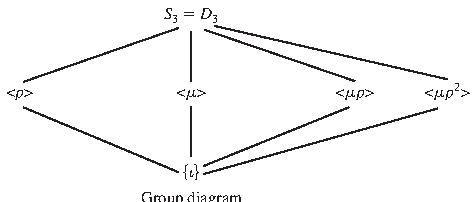
\includegraphics[width=0.651\linewidth,height=.8\textheight,keepaspectratio]{assets/p433_22.pdf}\end{center}
\end{BookFloat}

\begin{BookFloat}{answers-p433-29}
\begin{center}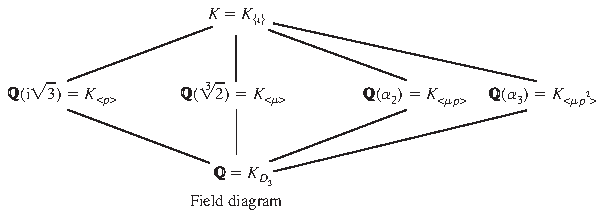
\includegraphics[width=0.824\linewidth,height=.8\textheight,keepaspectratio]{assets/p433_24.pdf}\end{center}
\end{BookFloat}

\BookExercise{13.}{The splitting field of \BookInline{(x^{3}- 1)\in \mathbb{Q}[x]} is \BookInline{\mathbb{Q} ( i \sqrt { 3 } )} and the group is cyclic of order 2 with elements\BookInline{:\iota,\allowbreak } where \BookInline{\iota } is the identity map of \BookInline{\mathbb{Q}(i\sqrt{3}),\allowbreak } and \BookInline{\sigma,\allowbreak } where \BookInline{\sigma (i\sqrt{3})= - i\sqrt{3}.}}

\BookExercise{5.}{\textbf{1. a} \BookInline{F} \textbf{c}\BookInline{.T} \textbf{e}\BookInline{.T} \textbf{g}\BookInline{.F} \textbf{i}\BookInline{.F}}

\BookExercise{25.}{\textit{Partial answer}\BookInline{:G(K/(E\vee L))= G(K/E)\cap G(K/L)}}

\end{BookBody}

% Source PDF page 434; original printed page 417
\BookSource{434}{417}
\BookNarrativefalse

\begin{BookBody}

\BookSectionTitle{47}{Illustrations of Galois Theory}

\BookExercise{5.}{The group is cyclic of order 5, and its elements are}

\begin{BookFloat}{answers-p434-3}
\begin{center}\begin{adjustbox}{max width=\linewidth}
\renewcommand{\arraystretch}{1.3}
\begin{tabular}{c|c|c|c|c|c}
 & $\iota$ & $\sigma_1$ & $\sigma_2$ & $\sigma_3$ & $\sigma_4$\\\hline
$\sqrt[5]{2}\to$ & $\sqrt[5]{2}$ & $\zeta\sqrt[5]{2}$ & $\zeta^2\sqrt[5]{2}$ & $\zeta^3\sqrt[5]{2}$ & $\zeta^4\sqrt[5]{2}$
\end{tabular}\end{adjustbox}\end{center}
\end{BookFloat}

where \BookInline{\sqrt { 2 }} is the real 5th root of 2.

\BookExercise{7.}{The splitting field of \BookInline{x^{8}- 1} over \BookInline{\mathbb{Q}} is the same as the splitting field of \BookInline{x^{4}+ 1} over \BookInline{\mathbb{Q},\allowbreak } so a complete description is contained in Example 47.7. (This is the easiest way to answer the problem.)}

\BookExercise{9.}{\textbf{. a} \BookInline{s_{1}^{2}- 2s_{2}} \textbf{b.} \BookInline{\frac { s _ { 1 } s _ { 2 } - 3 s _ { 3 } } { s _ { 3 } }}}

\BookSectionTitle{48}{Cyclotomic Extensions}

\BookExercise{3.}{\textbf{a.} 16 \textbf{b.} 400 \textbf{c.} 2160}

\BookExercise{5.}{30}

\BookExercise{7.}{\textbf{a}\BookInline{.T} \textbf{c}\BookInline{.F} \textbf{e}\BookInline{.T} \textbf{g}\BookInline{.T} \textbf{i}\BookInline{.F}}

\BookExercise{9.}{\BookInline{\Phi _{1}(x)= x- 1} \BookInline{\Phi _{2}(x)= x+ 1} \BookInline{\Phi _{3}(x)= x^{2}+ x+ 1} \BookInline{\Phi _{4}(x)= x^{2}+ 1} \BookInline{\Phi _{5}(x)= x^{4}+ x^{3}+ x^{2}+ x+ 1} \BookInline{\Phi _{6}(x)= x^{2}- x+ 1}}

\BookSectionTitle{49}{Insolvability of the Quintic}

\BookExercise{1.}{No. Yes\BookInline{,\allowbreak K} is an extension of \BookInline{\mathbb{Z}_{2}} by radicals.}

\BookExercise{3.}{\textbf{. a} \BookInline{T} \textbf{c}\BookInline{.T} \textbf{e}\BookInline{.T} \textbf{g}\BookInline{.T} \textbf{i}\BookInline{.F(x^{3}- 2x} over \BookInline{\mathbb{Q}} gives a counterexample.)}

\BookTextHeading{\textbf{APPENDIX}}

\begin{center}\begin{adjustbox}{max width=\linewidth}\BookInline{\displaystyle \begin{bmatrix} - 3 + 2i & - 1 - 4i \\ 2 & - i \\ 0 & - i \end{bmatrix}}\end{adjustbox}\end{center}

\begin{center}\begin{adjustbox}{max width=\linewidth}\BookInline{\displaystyle \begin{bmatrix} 2 & 1 \\ 2 & 7 \end{bmatrix}}\end{adjustbox}\end{center}

\BookInline{\Big[\Big]} \BookInline{\Big[\Big]}

\BookExercise{5.}{\BookInline{\begin{bmatrix} 5 & 16 & -3 \\ 0 & -18 & 24 \end{bmatrix}}}

\BookExercise{7.}{\BookInline{\begin{bmatrix} 1 & - i \\ 4 - 6i & - 2 - 2i \end{bmatrix}}}

\BookInline{\Big[\Big]} \BookInline{\Big[\Big]}

\BookExercise{9.}{\BookInline{\begin{bmatrix} 8 & - 8 i \\ 8 i & \quad 8 \end{bmatrix}}}

\BookExercise{11.}{\BookInline{\begin{bmatrix} 0 & - 1 \\ 1 & \quad 0 \end{bmatrix}}}

\BookExercise{13.}{\BookInline{- 48}}

\end{BookBody}
\ifdefined\BookMaster\let\BookFinish\relax\else\def\BookFinish{\end{document}}\fi\BookFinish
